%!TEX TS-program = xelatex
%!TEX root = ../../maxwell2018thesis.tex

\chapter[Information Retrieval]{Information Retrieval:\\A History and Background}\label{chap:ir_background}
Search today is ubiquitous, and is now commonplace due to the proliferation of the~\gls{acr:www} and commercial search engines\footnote{Or, as we refer to them in this thesis, \emph{retrieval systems.}}. Despite potential negatives that these technologies may bring -- turning us into \emph{shallow thinkers}~\citep{carr2008google_stupid}, for example -- retrieval systems today by and large make our lives easier, allowing us to find the proverbial needle in the haystack with minimal effort. These results are returned while honouring the implicit searcher contract by returning results in a timely manner.

%This is achieved while often attaining near perfect accuracy~\citep{vaughan2004new_measurements}.

\begin{figure}[h]
    \centering
    \vspace{4mm}
    \resizebox{1\hsize}{!}{
    
\includegraphics{figures/ch2-searchbox.pdf}}
    \label{fig:searchbox}
    \vspace{-5mm}
\end{figure}

The field of~\glsfirst{acr:ir} has been long established, and has led to the development of the associated technologies that make the contemporary retrieval systems that we use possible. One of the key developments was the creation of a \emph{de facto} approach to studying~\gls{acr:ir}, along with the various \emph{retrieval models} and means with which to evaluate their effectiveness. This chapter provides an overview of the history of~\gls{acr:ir}, before we move on to discussing the basics of what constitutes an~\gls{acr:ir} system. From there, we discuss the basics of~\gls{acr:iir} before moving onto how evaluation has evolved in the field, moving over a spectrum from the \emph{system} to the \emph{searcher.} Included in our discussion of the searcher are some of the current searcher models with which we improve upon, before we conclude the chapter with a discussion of the various measures used for evaluation of both system and searcher.

\section{A (Brief) History of Information Retrieval}\label{sec:ir_background:history}
While many associate the study of~\gls{acr:ir} with computers, the need to seek information in a quick and effective manner has existed throughout human history. In this section, we provide a very brief overview of some of the key advancements in what can be considered to be the study of~\gls{acr:ir} -- from library cataloguing approaches to contemporary retrieval systems.

 %This ranges from library indexing systems, to more contemporary retrieval systems that deal with the enormous volumes of content available on the~\gls{acr:www}.

\subsection{Libraries and Mechanisation}
Containing a large volume of books discussing a virtually unlimited range of categories, \emph{libraries} require the need for a means of organising (and thus easily locating) information with relative ease. \emph{Catalogues} provide such a way in which to do this, with ancient Greek poet Callimachus being the first person to create such an item in the third century BC~\citep{eliot2009companion}. A more recognisable approach to categorising content was devised by~\cite{dewey1891dcs} with the \emph{Dewey Decimal System}. The use of cards as an \emph{indexing system} was also considered by individuals such as~\cite{soper1920patent} who invented a system of providing information on what category a card belonged to based upon a punched hole.

In order to speed up the process of finding useful material, mechanisation was also extensively used. Allowing for searching at the rate of $600$ cards per minute, Luhn devised in the early 1950's a mechanised system which utilised punchcards and light. As stated by~\cite{sanderson2012history_of_ir}, this was also around the time that the term~\glsfirst{acr:ir} was used~\citep{mooers1950theory}. It was at this point that computer technology superseded mechanised systems, as outlined by~\cite{jahoda1961electronic_searching}.

\subsection{The Rise of Computers}
Computers now provide the underlying technologies with which we closely associate to a typical, contemporary~\gls{acr:ir} system.~\cite{sanderson2012history_of_ir} state that digital storage capacity (e.g. hard disks, and more recently, solid state storage) roughly doubles every two years. This claim is essentially analogous to the famous \emph{Moore's Law}~\citep{moore1965law}, which observes that the number of transistors in a processor (or other integrated circuit) doubles roughly every two years. Indeed, the speed at which modern day computers can search vast indexes and databases of content is vastly superior to traditional cataloguing approaches. These technological advances permit the near instantaneous returning of results, something that has become expected with today's retrieval systems.

Leading on from computers was the development of \emph{computer networks,} permitting the transmission of information between computers over potentially vast distances. With the development of the internet, the scene was set for the introduction of a technology that is extensively used today -- the~\glsfirst{acr:www}.

\subsection{The World Wide Web}
The distribution and ability to search for information over computer networks such as the internet was traditionally undertaken with legacy protocols such as \emph{Gopher.} Gopher would provide a series of options for a user to select (i.e. categorisation of content), akin to the traditional library cataloguing approaches described above.

\begin{figure}[t!]
    \centering
    \resizebox{1\hsize}{!}{
    
\includegraphics{figures/ch2-yahoo.png}}
    \caption[Screenshot of \emph{Yahoo!} Search, July 1998]{A screenshot of the landing page of \emph{Yahoo!}, as shown on July 5\textsuperscript{th}, 1998. Notice the link for the 1998 \emph{FIFA World Cup} that was taking place at the time the page was created. More central to this thesis is the inclusion of a list of page categories in conjunction with the now ubiquitous search box. Screenshot acquired from the \href{https://web.archive.org/web/19980705003104/http://www.yahoo.com}{\emph{Internet Archive}} (under fair use).}
    \label{fig:yahoo}
\end{figure}

The advent of the~\gls{acr:www} in the early 1990's brought about a new type of~\gls{acr:ir} system -- \emph{web search engines.} Regarded as the first experimental web search engine, \emph{JumpStation} was outlined by~\cite{mcbryan1994taming_tools}. In this system, \emph{anchor text} within \emph{hyperlinks} of~\gls{acr:html} pages could be exploited to aid the ranking of documents. However, popular search engines of the 1990's initially followed the categorisation approach hailing back from libraries, as illustrated in Figure~\ref{fig:yahoo} with a screenshot of \emph{Yahoo!} from 1998. This categorisation approach on the Yahoo! front page ties in with the surfing paradigm described back in Chapter~\ref{chap:intro}. However, as the volume of information on the~\gls{acr:www} began to increase, this way of presenting information became impractical. As such, it was not long before the now contemporary paradigm of search took ahold, allowing individuals to pose their own \emph{queries}. Work examining the retrieval systems that we utilise today can trace their roots to the study of~\glsfirst{acr:ir}. As we will discuss throughout the remainder of this chapter, work includes aspects such as the basic components of a retrieval system, and approaches used for the evaluation of such systems.

\section{Information Retrieval Basics}
A contemporary~\gls{acr:ir} system is expected by the searchers that use it to return results that can be considered \emph{relevant} to addressing their information need. These results should be \emph{ranked} in a decreasing order of relevance. This was originally hypothesised by~\cite{luhn1957ranking_query}, and succinctly expressed by~\cite{robertson1977prp}.

\begin{quote}
    ``A [reference] retrieval system should rank references in the collection in order of their probability of relevance to the request, or of usefulness to the user, or of satisfying the user.''
    \attrib{\cite{robertson1977prp}}
\end{quote}

Such a system would search through collection(s) of \emph{unstructured} or \emph{semi-structured} data (such as collection of web pages or documents, or even images or videos for \emph{multimedia retrieval}) before returning potential matches to the searcher.

\blueboxheader{Unstructured and (Semi-)Structured Data}
A key difference between a traditional database system -- or~\gls{acr:rdbms} -- and an~\gls{acr:ir} system is the type of data that they consider. While a~\gls{acr:rdbms} considers \emph{structured data,} an~\gls{acr:ir} system in contrast considers \emph{semi-structured data}, as illustrated in Figure~\ref{fig:structured_data}. With an~\gls{acr:ir} system, such a premise for structured data does not exist.\footnote{This may be a slight misnomer; schemas can be used for an~\gls{acr:ir} system index when considering \emph{fielded retrieval}. For example, a collection of newspaper articles may contain a title and body -- but within the fields, the data is unstructured.} Semi-structured data such as an~\gls{acr:html} page contains a series of \emph{elements} (e.g. section headers represented within header elements such as \texttt{<h1>}, \texttt{<h2>}, \texttt{<h3>} up to \texttt{<h6>}), but the text within these elements is largely of an unstructured nature. The unstructured data can contain information such as dates or entities (terms describing a real-world object and/or location, such as \texttt{canberra} or \texttt{dropbear}, and can be -- as it is probably written in a natural language -- ambiguous. As such, examining this unstructured data presents a major challenge to researchers.

\begin{figure}[t!]
    \centering
    \resizebox{1\hsize}{!}{
    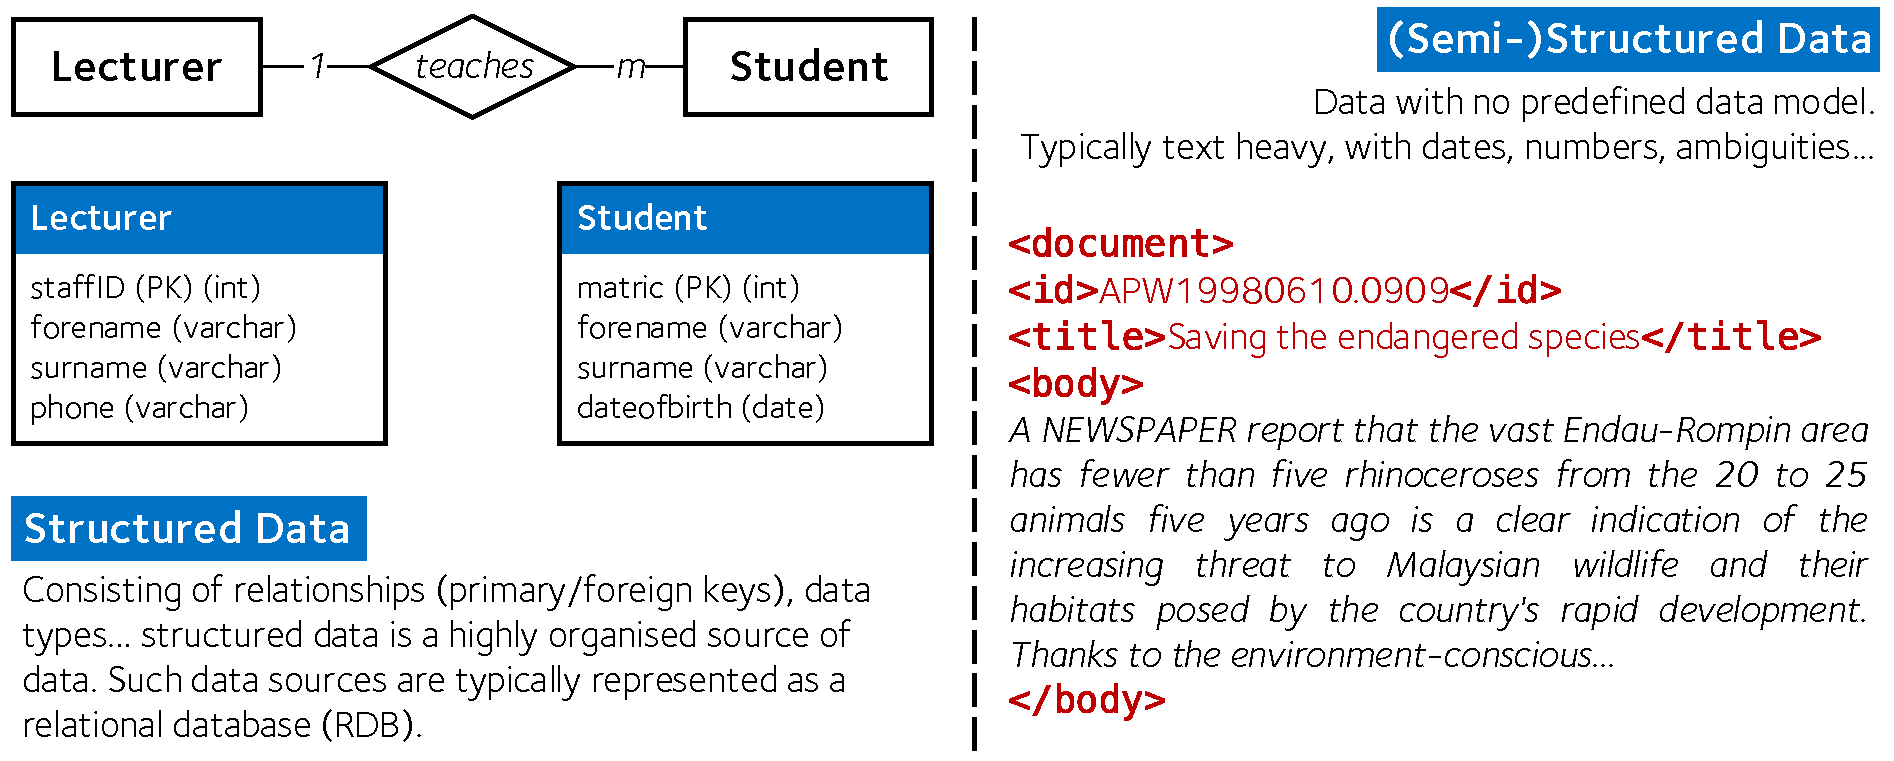
\includegraphics{figures/ch2-structured.pdf}}
    \caption[Structured and (semi-)structured data]{Examples of structured and (semi-)structured data. On the left is a structured~\gls{acr:rdbms} schema, represented in \emph{compressed Chen notation}~\citep{chen1976notation}. Different types can be specified for each field, representing data in a structured way. On the right, semi-structured data, using a document from a newswire collection. Note the semi-structured component at the top of the document (containing an identifier and title), and the unstructured body text.}
    \label{fig:structured_data}
\end{figure}

Being able to effectively sift through large volumes of unstructured data led to the development of retrieval systems. Consisting of a number of key components, the basic process of a retrieval system -- along with the \emph{users,} or \emph{searchers} that utilise such systems -- can be seen in Figure~\ref{fig:irs}. Core to the wider system is the \blueboxbold{retrieval engine}, of which many \emph{experimental}\footnote{\cite{rijsbergen1979ir} defines a difference between \emph{operational} and \emph{experimental}~\gls{acr:ir} systems. A majority of individuals will only ever interact with an operational system (such as Google). The work in this thesis however focuses more on experimental~\gls{acr:ir} systems, and the methodology employed to compare different experimental retrieval systems against each other.} retrieval engines can be selected based upon the requirements and existing infrastructure available. Examples include \emph{Lemur/Indri,} \emph{Lucene for~\gls{acr:ir}}, \emph{Okapi,} the \emph{Terrier~\gls{acr:ir} platform,} \emph{Wumpus} and \emph{Zettair.} Common to all systems are three key inputs, which are:

\begin{itemize}
    \item{an \blueboxbold{index} of documents, a specially crafted data structure used for the fast lookup of documents derived from a source collection, or \emph{corpus};}
    \item{a \blueboxbold{retrieval model} that scores and identifies documents that may constitute as relevant to what is being searched for; and}
    \item{a \blueboxbold{query}, the construct that represents a given \emph{information need} by a searcher -- or one of several queries issued in a \emph{batch environment.}}
\end{itemize}

\begin{figure}[t!]
    \centering
    \resizebox{1\hsize}{!}{
    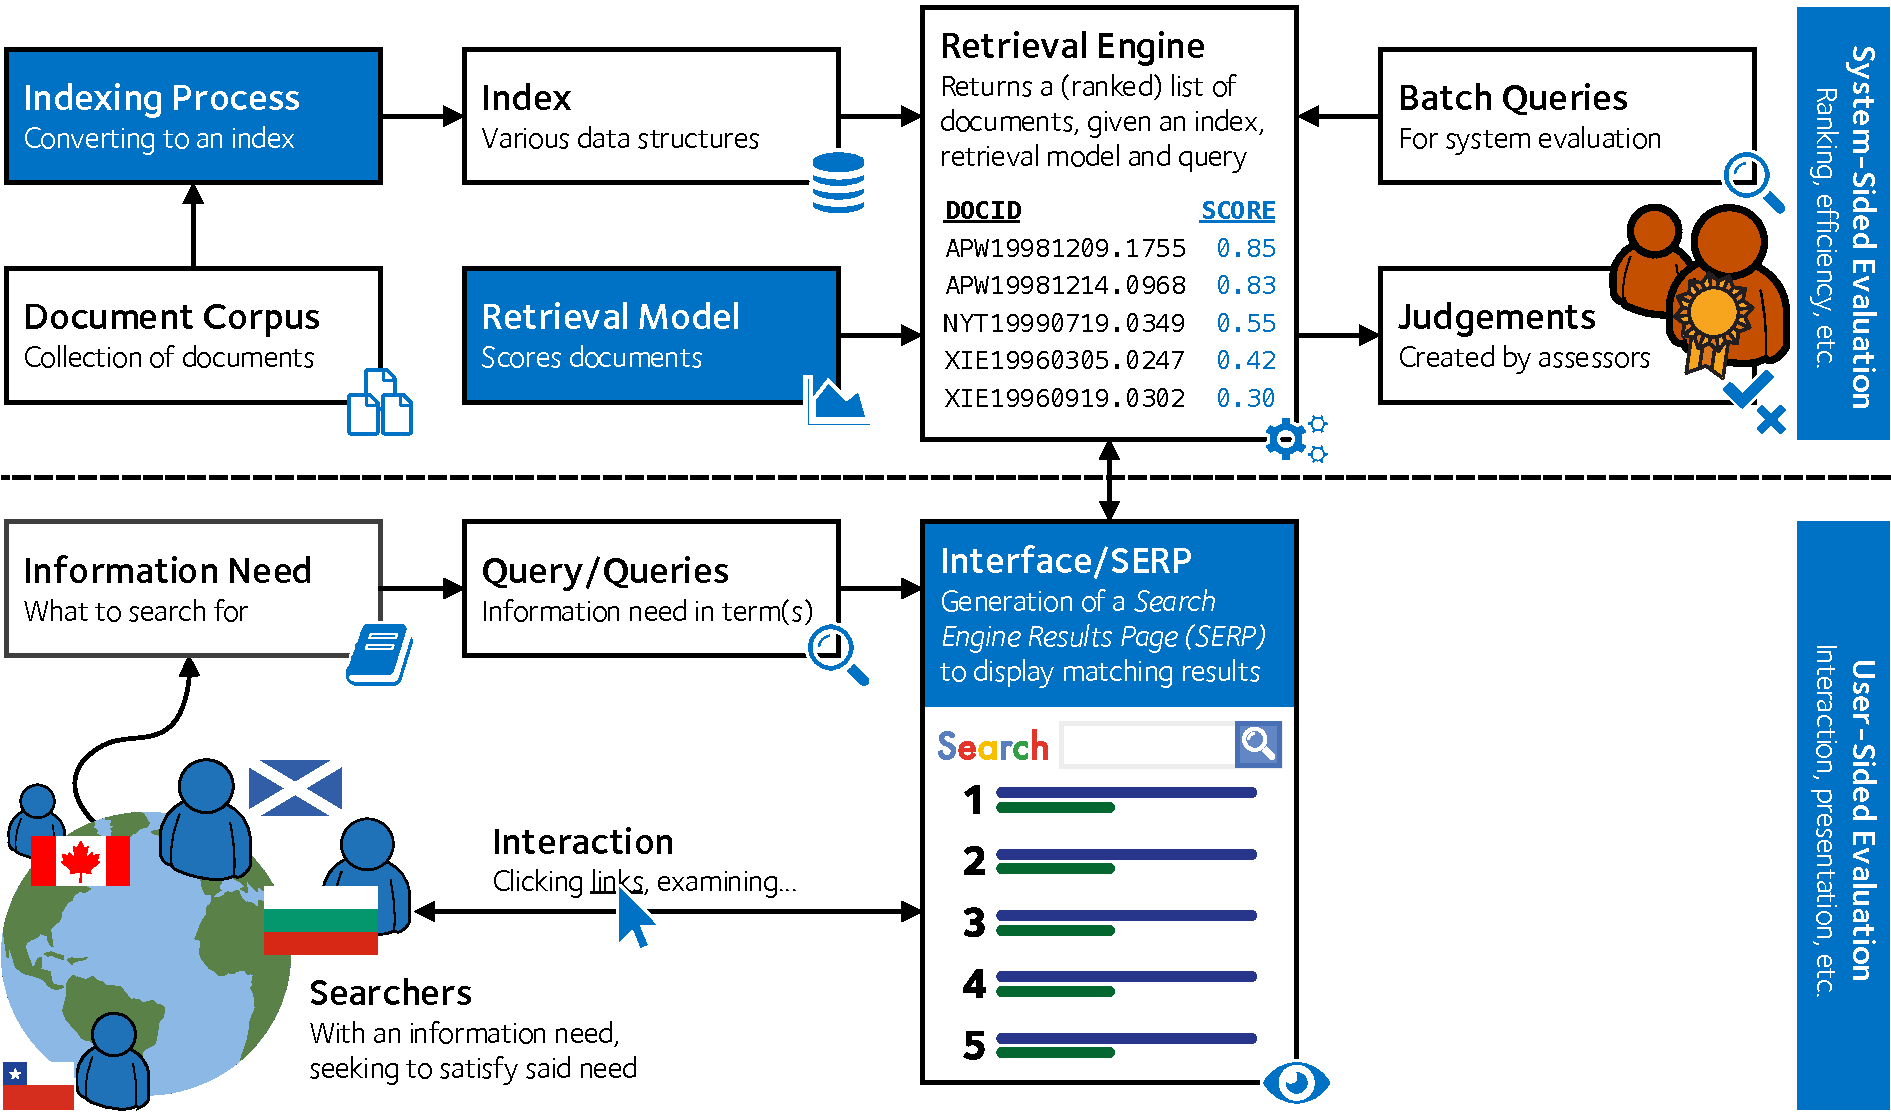
\includegraphics{figures/ch2-irs.pdf}}
    \caption[Basics of an experimental retrieval system]{The core components of a retrieval system, including the key processes that we discuss in this chapter, highlighted in blue boxes. Central to the discussion in this chapter is the delineation between \emph{system-sided} and \emph{user-sided} evaluation, with both clearly separated in this figure by the dashed line. On the top, system-sided aspects include the \emph{retrieval engine, retrieval model} and \emph{index.} Below, user-sided aspects include the \emph{interface}, \emph{interactions} that take place with said interface, and constructs such as the searcher's \emph{information need} and derived \emph{query/queries.}}
    \label{fig:irs}
\end{figure}

The retrieval engine combines these inputs to yield an output. This is a ranked list of documents\footnote{Depending upon the retrieval model used, ranking may or may not occur -- refer to Section~\ref{sec:ir_background:basics:models} for more information.} that the retrieval model believes are relevant to the given query. This is often called the \emph{matching process.} The retrieval model is responsible for performing the matching of documents from an index. This index typically constitutes a number of different data structures that are generated through the \emph{indexing process}, where a source document corpus is processed. As highlighted by the blue boxes in Figure~\ref{fig:irs}, we discuss the indexing process and various retrieval models in this chapter, explained in Sections~\ref{sec:ir_background:basics:indexing} and~\ref{sec:ir_background:basics:models} respectively. These components are all considered as \blueboxbold{system-sided} aspects of the wider retrieval system, with evaluation of system-sided aspects concerning the quality of returned rankings, how efficient the retrieval engine is, etc.

The system-sided aspects only however tell part of the wider retrieval process. We build retrieval systems to help searchers satisfy their information need -- and hence the study of~\gls{acr:iir} is devoted to considering the interactions between the searcher and retrieval system. While we discuss more \blueboxbold{user-sided} aspects later on in this chapter (Section~\ref{sec:ir_background:user}), searchers, given an information need, will issue one or more queries, and \blueboxbold{interact} with the presented interface~\citep{ingwersen2005theturn}, or~\glsfirst{acr:serp} (refer to Section~\ref{sec:ir_background:user:iir:serp}) -- with the goal of satisfying said information need. User-sided evaluation is also considered extensively in this thesis, with aspects such as the interactions that take place, how presentation of results affects behaviour, etc. all being considered.

Before discussing user-sided aspects, we now turn our attention to the system-sided components of the wider retrieval system: the indexing process, and various retrieval models that are commonly employed.

\subsection{The Indexing Process}\label{sec:ir_background:basics:indexing}
The process of indexing takes into account the conversion of a collection of documents (or corpus) into a data structure that facilitates fast, full-text search -- a key requirement of any retrieval system. This full-text search is typically undertaken in milliseconds, with the goal of finding documents that will be relevant to a given query (and thus information need). The additional storage space and management requirements to maintain an index of documents is considered to be a necessary tradeoff to guarantee timely responses to searcher queries.

As illustrated in Figure~\ref{fig:inverted}, the indexing process can be split into three main steps:

\begin{itemize}
    \item{gathering the corpus of documents to be indexed;}
    \item{performing pre-indexing data preparation; and}
    \item{creating the various data structures that constitute an index.}
\end{itemize}

Experimental corpora are available for use with batch experimentation, typically for \todo{various evaluation forums.} For operational retrieval systems, data is collated by other means. For example, web search engines employ a \emph{web crawler} to examine pages on the~\gls{acr:www}, and accumulates more content by following the~\glsplural{acr:www} hyperlink structure. Google's crawler, \emph{Googlebot,} regularly crawls high impact websites to ensure that the associated index is continually refreshed with up to date information.

\begin{figure}[t!]
    \centering
    \resizebox{1\hsize}{!}{
    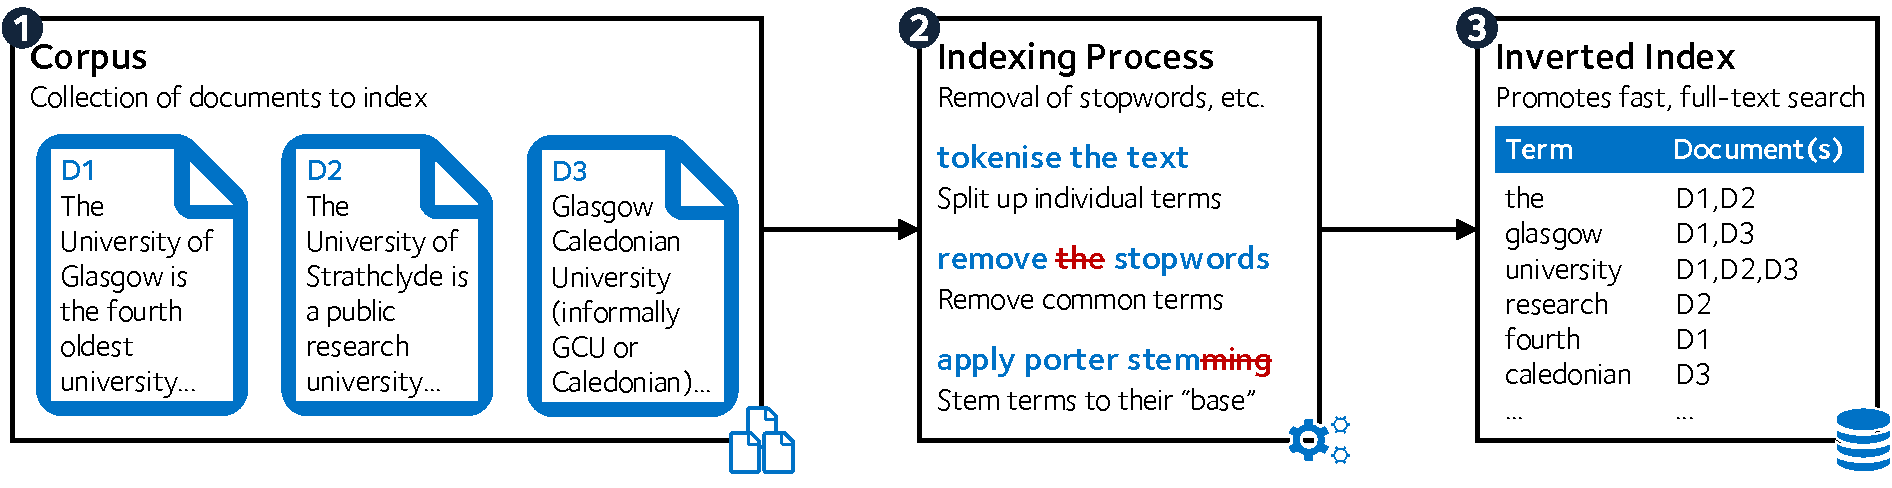
\includegraphics{figures/ch2-inverted.pdf}}
    \caption[Illustration of an \emph{inverted index}]{A demonstration of an \emph{inverted index}, with three source documents for comparison. Depending upon the requirements of the~\gls{acr:ir} system, the indexing process may vary; all classical~\gls{acr:ir} systems however rely upon some form of inverted index.}
    \label{fig:inverted}
\end{figure}

An index will contain an entry for each processed document, along with a \emph{vector of terms} that are present within said document. This is known as the \emph{forward index.} A retrieval system however needs to support fast full-text search, matching terms from a searcher's query to one or more documents within the index. To support faster query matching, the most simplistic approach is to simply \emph{invert} the index, such that the lookup of the index then corresponds to individual terms, not individual documents. A \emph{vector of documents} can then be provided for each term, yielding much faster access to a potential list of documents. An example of an inverted index is provided in Figure~\ref{fig:inverted}. The source corpus in this example illustration consists of three documents, and the resultant inverted index is shown. The set of documents retrieved can then be sent to a retrieval model for ranking.

Before a document is indexed however, a number of pre-indexing steps usually take place. Three of the most common processes involved within such a pipeline include \emph{tokenisation,} \emph{stopword removal} and \emph{stemming.}

\subsubsection{Tokenisation}
Put simply, tokenisation is the process of \emph{parsing} a source document, and splitting the data within the document into a number of individual \emph{tokens} that may be subsequently indexed. A token is considered a sequence of characters, grouped together to be semantically useful for processing its given document. While we do not go into greater deeper about the process of tokenisation, there are many challenges to this process -- such as \emph{word boundary ambiguity}. While parsing an English or Latin-based document may be relatively straightforward (with spaces representing \emph{word boundaries}), what about other languages, such as Chinese or Japanese? Considering what words a potential searcher of a retrieval system may use to search with may be a potential pathway for finding a solution to this problem.

\subsubsection{Stopword Removal}
Stopword removal is another popular choice for indexing document collections for an experimental~\gls{acr:ir} system. Illustrated in Figure~\ref{fig:inverted}, extremely common words which would appear to have little value in selecting documents matching a searcher's query (that is, \emph{non-discriminative} words) can simply be removed from a document's vocabulary entirely. Examples of such words could be \emph{the}, \emph{a}, or \emph{did}, or even a complete phrase from the famous soliloquy of William Shakespeare's \emph{Hamlet:} \emph{``to be or not to be''.} Such words are regarded as \emph{stopwords}. Some experiments consider a small list of stopwords, while others consider a larger list, with larger lists often significantly reducing the size of an indexed corpus~\citep{manning2008ir}. Indeed, it was argued by~\cite{fox1992stopwords} that larger lists ``are advisable''.

While stopword lists may be manually crafted under particular scenarios, automatic extraction from a document corpus is perhaps a more common practice. A simple approach would be to count the \emph{term frequency} for each term within a corpus, and sort the resultant list in descending order, selecting some top \emph{k} of the most frequently occurring terms. Readily available lists are also available.~\cite{rijsbergen1979ir} for example produced a list of 250 terms, with~\cite{francis1985stopwords} demonstrating a list of 425 stopwords from the \emph{Brown corpus}\footnote{The \emph{Brown corpus} was a collection of documents representing (then) contemporary American English, compiled by William Francis and Henry Ku\v{c}era -- refer to~\cite{francis1979brown_manual} for more information.}. For the experiments detailed in this thesis, \emph{Fox's classical stopword list}~\citep{fox1992stopwords} is used, consisting of 421 terms. Such an approach may be considered fine, but stopwords lists do vary from collection to collection, as stated by~\cite{lo2005automatically}.

Issues of course also exist with the removal of stopwords. Removing stopwords from a query may decrease processing time, but what if all terms within a query are stopwords? The resultant query passed to the retrieval engine could contain zero terms! As such, commercial retrieval systems are less likely to employ stopword removal to counter such an occurrence~\citep{manning2008ir, dolamic2010stopword}. Techniques such as compression may be employed to keep the size of the resultant index down. Queries such as \texttt{`to be or not to be'} may well contain some semantical meaning. Like tokenisation, there is often more to this problem than meets the eye.

\subsubsection{Stemming}
Another common pre-indexing process is \emph{stemming} (also called \emph{lemmatisation).} This is the process of reducing inflected -- or sometimes derived -- words from their \emph{word stem, base} or \emph{root.} For example, given the terms \texttt{fisher}, \texttt{fished} and \texttt{fishing}, reducing each of these terms to their respective word stem would result in \texttt{fish}. Essentially, stemming allows one to group words together with a similar, basic semantical meaning. This provides the advantage of reducing the size of an index, with fewer terms to index. A further benefit may be the potential increase in the number of possible matches that can be found with a stemmed set of query terms, increasing the retrieval system's \todo{\emph{recall.}}

The concept of stemming has been studied since the 1960's, with the \emph{Porter stemmer}~\citep{porter1980algorithm} emerging over time as empirically the most effective.\footnote{The Porter stemming algorithm is not provided in this thesis; refer to~\cite{porter1980algorithm} for an in-depth explanation of the algorithm.} Comprised of a series of linguistic rules, the \emph{measure} of a word can be considered, where \emph{``loosely checking the number of syllables to see whether a word is long enough that it is reasonable to regard the matching portion of a rule as a suffix rather than as part of the stem of the word.''}~\citep{manning2008ir}. Porter stemming is utilised in the indexing process for the work reported in this thesis; other stemmers do exist, with examples including the original single pass stemmer devised by~\cite{lovins1968development}, and the Krovetz stemmer~\citep{krovetz1993stemming}.

Issues such as \emph{overstemming} can impact upon the performance of a retrieval system. This is when terms are reduced back too far to the point that it loses meaning -- and can thus negatively affect the results returned. Terms like \texttt{universe}, \texttt{university} and \texttt{universal} when stemmed will be reduced to \texttt{univers}. While the three original terms may be etymologically linked, their modern meanings are however very different. If stemming is applied like so, documents containing both \texttt{universe} and \texttt{university} could be returned. While we do not go into depth into the solutions to this problem in this thesis, one potential solution is to consider the \emph{$n$-gram} context of a given term, allowing the retrieval system to thus select the correct step for the term~\citep{mcnamee2005stemminggrams}.

\subsection{Retrieval Models}\label{sec:ir_background:basics:models}
Given a generated document index and a searcher's query, the next part of the process is retrieval, or \emph{matching.} For this, a number of mathematically-based \emph{retrieval models} have over the years been developed that attempt to operationalise the notion of relevance. Such models provide us with a means for discussion and further refinement. They also provide us with the blueprint from which we operationalise a retrieval system~\citep{hiemstra2009ir_models}. The usefulness of such a model can be subsequently tested via experimentation and evaluation.

Several different types of retrieval model have been defined, ranging from the relatively simplistic, to the more complex. More complex approaches not only define a notion of what documents would be considered relevant, but also to what \emph{degree} that is so. This section considers four main retrieval model families, including:

\begin{itemize}
    \item{the \emph{boolean model;}}
    \item{the \emph{vector space model;}}
    \item{\emph{probabilistic models;} and}
    \item{more recent \emph{language models.}}
\end{itemize}

While not totally exhaustive -- approaches such as contemporary \emph{neural~\gls{acr:ir} models}~\citep{mitra2017neural_ir} are not considered here, for example -- this broad overview provides a solid understanding of the developments of such models, and the benefits and disadvantages of each approach. We focus the discussion of each retrieval model with an emphasis on how it can potentially influence the stopping behaviours of searchers.

\subsubsection{Boolean Model}
Cited as the first formally defined~\gls{acr:ir} retrieval model, the boolean model is also the most likely one to be criticised~\citep{hiemstra2009ir_models}. The model employs operators of mathematical logic as defined by George Boole~\citep{boole1847mathematical}, or \emph{set theory.} Boole defined three basic operators: \texttt{AND}, yielding a logical product between two sets; \texttt{OR}, yielding the logical sum between two sets; and \texttt{NOT}, yielding the logical difference.

\begin{figure}[t!]
    \centering
    \resizebox{1\hsize}{!}{
    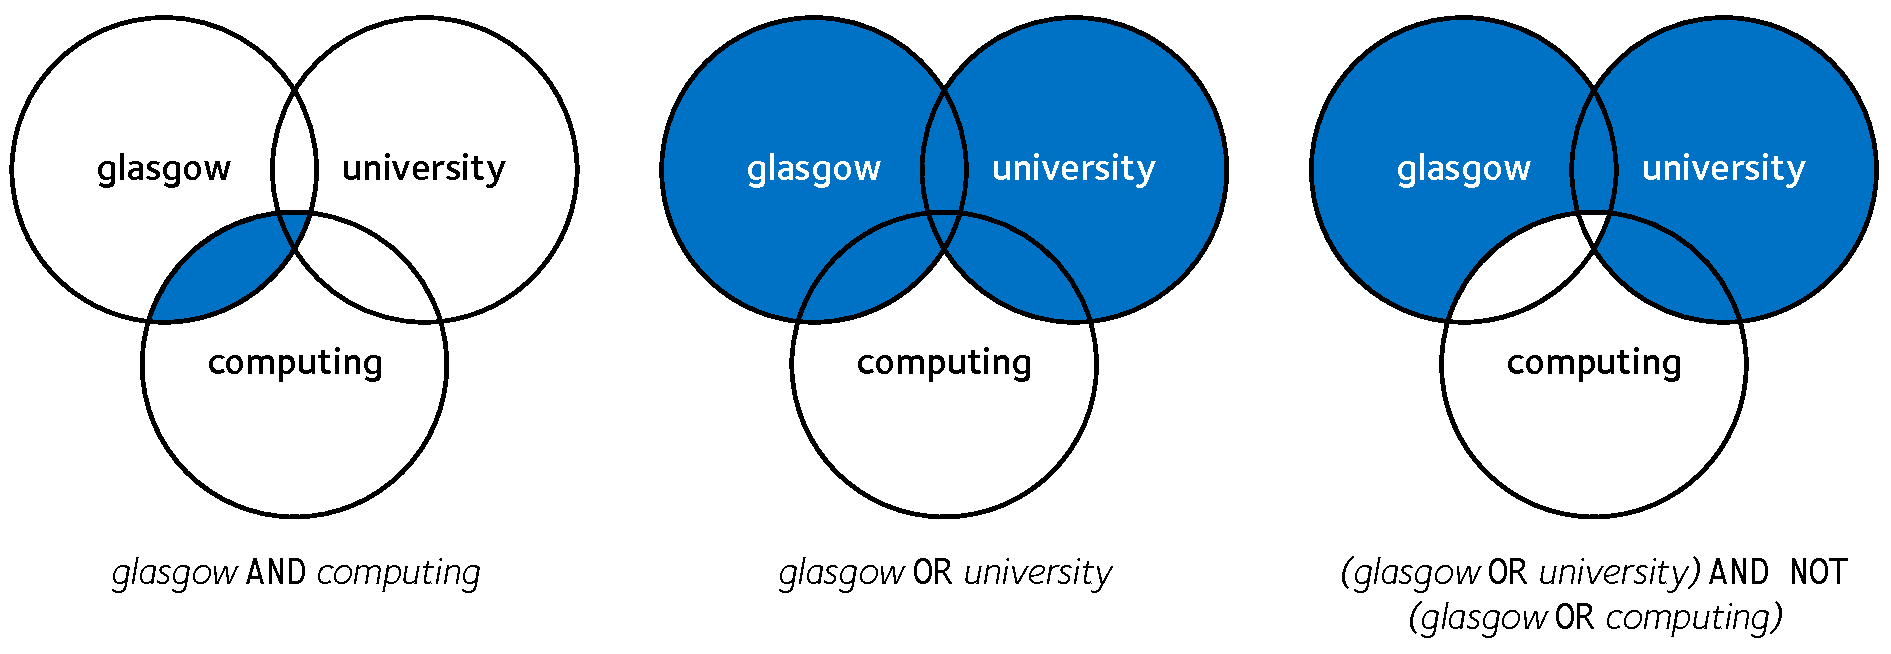
\includegraphics{figures/ch2-boolean.pdf}}
    \caption[Venn diagrams illustrating boolean retrieval]{An example illustration of the boolean retrieval model, using the query terms \texttt{glasgow}, \texttt{university} and \texttt{computing}. Each disc represents the set of documents containing that particular term. In the figure, three Venn diagram examples are provided, demonstrating the key logical operators used (\texttt{AND}, \texttt{OR} and \texttt{NOT}). Areas in blue are returned in the example boolean query provided underneath each Venn diagram.}
    \label{fig:boolean}
\end{figure}

By considering an individual query term and an unambiguous set of documents, logical operations can be applied to retrieve a set of documents. For example, the query term \texttt{glasgow} will yield a set of all documents containing the term \texttt{glasgow}, yet the query \texttt{NOT glasgow} will retrieve the set of documents that \emph{do not} contain any mention of the term \texttt{glasgow}. These results of applying logical operators between different sets can be illustrated through a \emph{Venn diagram,} where each set of documents is represented as a disc. Figure~\ref{fig:boolean} provides an example of such diagrams, using \texttt{glasgow university computing} as an example.

Despite its relative simplicity, there are major limitations to the exact match approach. First, when considering the boolean query, there is no notion of term importance -- every term has equal weighting. Querying utilising logic rules also appear as relatively unnatural representations of the searcher's information need. Indeed, as an information need becomes more complex, the corresponding boolean query can grow to be disproportionally large and cumbersome to interpret. As documents either belong to a set or not, a document is considered to be either relevant \texttt{(TRUE)} or not \texttt{(FALSE)}. As such, one cannot estimate a degree to how relevant a document would be to the searcher's query, and thus results are provided to the searcher in an unranked manner.

Returning an unranked set of documents would appear as an alien concept to searchers of contemporary retrieval systems -- one would assume that the document presented first would be the document considered to have the greatest relevance, as per the underlying retrieval model. This would make it difficult for a searcher to obtain some notion of how many results he or she should examine before stopping -- no ranking means all returned documents are of equal importance. 

\begin{figure}[h]
    \centering
    \vspace{4mm}
    \resizebox{1\hsize}{!}{
    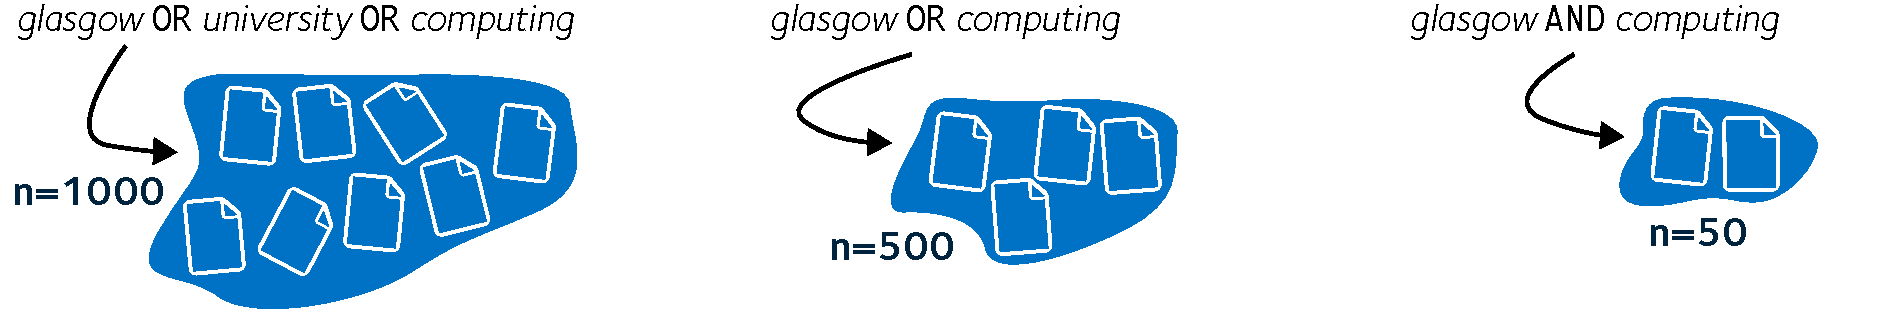
\includegraphics{figures/ch2-boolean-reduce.pdf}}
    \label{fig:searchbox}
    \vspace{-5mm}
\end{figure}

Instead, a searcher utilising a boolean retrieval system will often find an initial exploratory query will return a large set of documents, too many to examine each in sufficient detail. Rather, what a searcher will do is gradually reformulate their query -- like in the illustration above -- until the document set returned is of a manageable size, and small enough to process. This is an inherently different kind of stopping behaviour from the examples provided thus far in this thesis that assumes documents are presented in a \emph{ranked} list, with some notion of a \emph{depth} at which a searcher would stop.

Despite not being required in contemporary retrieval systems, many systems still do provide support for crafting a boolean query for when returning a good set of results is difficult. Boolean queries may also be of use where ambiguity exists within a searcher's query, and clarification is required to eliminate a set of non-relevant documents. Indeed, boolean queries still find considerable traction in professional search systems, such as patent search. Here, missing an existing, relevant patent may be incredibly costly -- here, \emph{recall} is preferred over \emph{precision}, as discussed in \todo{Section~\ref{}.}

\subsubsection{Vector Space Model}
With major weaknesses present in the boolean retrieval model, work then progressed to develop more advanced approaches that mitigated the issued raised above.~\cite{luhn1957ranking_query} hypothesised that a searcher, when wishing to search for documents addressing their information need, should prepare a document that is similar to the documents being sought after. By comparing documents against this \emph{representative} document, a retrieval system could then begin to deduce what other documents would be useful, and by \emph{what margin.}

The vector space model proposed by~\cite{salton1975vsm} incorporates the principles as outlined by~\cite{luhn1957ranking_query}. These basic principles are operationalised by representing queries and documents within Euclidean geometry, where both are represented as vectors in multi-dimensional space. The notion of how close documents appear to each other denotes the relevance of a document.

\begin{wrapfigure}[13]{r}{0.45\textwidth}
    \begin{center}
    \vspace*{-10mm}
    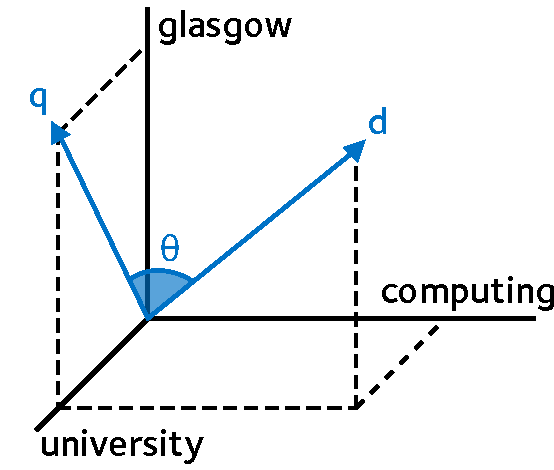
\includegraphics[width=1\textwidth]{figures/ch2-vector.pdf}
    \end{center}
    \vspace*{-4mm}
    \caption[Vector space model (cosine similarity)]{An illustration of the vector space model in Euclidean space, with each term representing a dimension. Here, the cosine similarity between query \emph{q} and document \emph{d} is shown.}
    \label{fig:vector_space}
\end{wrapfigure}

The vector space model has been very popular, as it provides an intuitive means for addressing the overarching problem of a retrieval system. It can also incorporate methods such as \emph{term weighting,} which has been shown to improve retrieval effectiveness~\citep{croft2010search}. Furthermore, as queries and terms ad represented in Euclidean space, vector similarity methods can be employed to determine relevance. While many approaches have been trialled, empirical evidence have favoured \emph{cosine similarity}~\citep{croft2010search}. This is illustrated in Figure~\ref{fig:vector_space}. Using such an approach allows one to then compute the degrees of relevance, meaning that matched document can be returned in a ranked order. The ability of providing a ranking then permits searchers interacting with the results list to decide at what depth they should stop examining them. In other words, the ranking provides searchers with an \emph{estimate} as to when they should stop, or when the scores assigned to documents from a particular ranking begin to fall below an acceptable threshold.

In order to understand the basic workings of the vector space approach, let us consider a query, $Q$, with each of its constituent terms placed within a term vector in $t$-dimensional space, leading to $Q = (q_1, q_2, q_3,\dotsc, q_{it})$. Consider also a document, $D_i$, with terms from the document again represented in $t$-dimensional space, yielding $D_i = (d_{i1}, d_{i2}, d_{i3},\dotsc, d_{it})$. From this notation, $d_{ij}$ represents the \emph{term frequency (TF)} of term $j$ appearing in document $i$. With each term represented as a separate dimension within Euclidean space, a weighting scheme can be subsequently applied to emphasise or understate more discriminative or less discriminative terms, respectively. By applying weighting schemes, the vector space model ranks documents which promotes terms that are more discriminative, thus improving the quality of the returned ranked list.

Term frequency is one of many different term weighting schemes that have been trialled over the years in~\gls{acr:ir} research. Perhaps one of the best and widely used schemes is \emph{inverse document frequency (IDF)}, proposed by~\cite{sparck1972statistical}. Here, the frequency of a term is normalised against the length of a given document. In the words of its creator, IDF allows for one to define the specificity of a term as \emph{``an inverse function of the number of documents in which it occurs.''}~\citep{sparck1972statistical}. This is useful as non-discriminative terms that occur frequently within an index (e.g. \texttt{the}) would have a small weighting applied, with the inverse happening for more discriminative terms, better able to describe a given document.

TF and IDF are typically combined together as a measure of both term appearance and importance, under an approach called \emph{TF-IDF}. For a given term $k$, one can calculate a TF-IDF score with the following equation:

\begin{equation*}
tf_{i,k} \cdot idf_{k} = \frac{f_{i,k}}{\sum_{j=1}^{t} f_{i,j}} \cdot log \frac{N}{n_k}.
\end{equation*}

Above, $f_{i,k}$ is the frequency of term $k$, $N$ is the number of documents in the collection used, and $n_k$ is the number of documents in which term $k$ appears at least once.


\subsubsection{Probabilistic Models}
The next major development were probabilistic retrieval models, defined to estimate the likelihood of a document being relevant to a given query. One of the most well known ranking principles, known as the \emph{Probability Ranking Principle (PRP)} -- defined by~\cite{robertson1977prp} -- who in turn attributed the development to~\cite{cooper1971relevance} -- states the following:

\begin{quote}
\emph{``If a reference retrieval system's response to each request is ranking of the documents in the collections in order of decreasing probability of usefulness to the user who submitted the request, where the probabilities are estimated as accurately as possible on the basis of whatever data has been made available to the system for this purpose, then the overall effectiveness of the system to its users will be the best that is obtainable on the basis of that data.''}
\attrib{\cite{robertson1977prp}}
\end{quote}

Essentially, this states that documents that are considered more likely to be relevant than non-relevant should be retrieved -- or where $P(R|D) < P(\overline{R}|D)$. However, while the PRP lays the much of the foundation from which probabilistic models have been derived, it does not provide its own concrete implementation of such a model.

Perhaps one of the most widely used derived models if \emph{Okapi BM25}~\citep{robertson1995trec3}. Indeed, this retrieval model has had considerable impact upon the~\gls{acr:ir} community, and is still used extensively today. BM25 provides a solid baseline for contemporary research, and is indeed the retrieval model employed in the experimentation discussed in this thesis, primarily for its effectiveness and popularity. Such a model, like the vector space model, again provides a ranking for documents returned -- and thus provides searchers with a gauge as to how relevant a document can be, given its ranking. Thus, it intrinsically provides a cue as to the depth at which a searcher should stop.

\subsubsection{Language Models}
The final retrieval model family that we discuss are language models, closely related to the probabilistic model we define above. Indeed, while such probabilistic models have been demonstrated to perform well empirically, adapting the PRP and subsequent developments to more advanced approaches has been difficult and is generally not intuitive~\citep{hiemstra2000language_modelling} -- the interpretation offered by probabilistic models may be considered loose, and is not always theoretically principled~\citep{whiting2015phd}. This has led to the development of more formalised statistical language modelling approaches, as defined in the fields of \emph{Natural Language Processing (NLP)}, for example~\citep{lavrenko2001language_models}.

Given the strong rooting in the principles of language and associated fields, language models provide a solution to the so-called \emph{bag of words}~\citep{harris1954distributional} concept that a majority of preceding retrieval models subscribe to. Put simply, this concept considers each document and query as a bag of words, meaning that the ordering of terms loses any significance. While a simplifying assumption, losing the ordering of terms means that semantic meaning and grammar rules are lost -- and thus a retrieval engine employing a model using this simplifying assumption may lose key meanings, and subsequently retrieval effectiveness will suffer.

Essentially, a language model is a probability distribution over strings of text. Given a string of text (i.e. a searcher's query), how likely is it that the given query appears in a given \emph{language}? Each document provides its own language, where we consider all possible phrases that the author of a document could have written when creating said document. Of course, some phrases are more likely than others. For example, the phrase \texttt{rain in glasgow} is more likely to appear in a document (in that order) than the seemingly random assortment of terms \texttt{purple monkey dishwasher}\footnote{If you ever watched \emph{The Simpsons}, you might disagree with this statement.}. Given this, and conceptualising a searcher's query in much the same fashion, we can produce a probability distribution $P(Q|D)$, concerning the probability of observing query $Q$ during some form of sampling within the language model of document $D$.

The most simplistic approach to language modelling is the \emph{unigram} approach, where each term within a document and/or query are considered in isolation, which subscribes to the aforementioned simplifying bag of words concept. Essentially, such an approach provides a probability distribution over the words appearing in the language. Higher order \emph{grams} such as \emph{bi-grams} and \emph{tri-grams} begin to consider more the place in which terms appear with respect to others, and thus the semantic meaning defined by this positioning begins to be taken into account within the probability distribution. When considering a document, the more a document discusses a particular topic, the more likely one would begin to observe terms about that topic in said document. When a term is not mentioned in a document, smoothing can be applied (given the wider collection the document is part of) to avoid a zero probability when calculating the probability of terms permitting the partial matching of queries where not all terms appear within a target document.

\section{From System to Searcher}\label{sec:ir_background:user}
So far in this chapter, we have provided a background on several key developments in the field of~\gls{acr:ir}. However, these developments are focused exclusively on the \emph{system.} Indeed, the overall goal of a retrieval system is to satisfy the information needs of the \emph{user.} Satisfying this information need is key to a successful retrieval system.

In this section, we discuss a line of research that moves primarily from considering the system to a more extensive examination of the searcher and his or her interactions with a retrieval system. This is examined in the study of~\glsfirst{acr:iir}. However, before discussing the~\gls{acr:iir} process, we must first consider in more detail the paradigms that have been extensively used in traditional, \emph{system-sided} ~\gls{acr:ir} research. These paradigms have been the underpinnings of scientific methodology for many decades, and can be largely considered to be largely na\"{i}ve of the behaviour of a searcher. After discussing these paradigms, we then move onto our discussion of~\gls{acr:iir}, emphasising the \emph{spectrum} of research between the system-sided and user-sided extremes. This then leads onto the concept of \emph{searcher models} that attempt to capture the high-level, cognitive processes that searchers undertake.

% Considering the user -- what is IIR?
% Core to their experience is the SERP as shown above.
%
% Kelly has a spectrum of studies that consider the searcher.
%
% From system-focused, to user focused.
%
% Explain the IIR process.
% Talk about the different kinds of tasks that people do.

\subsection{Experimental Paradigms}\label{sec:ir_background:paradigms}
The methodology behind the majority of classical~\gls{acr:ir} research has focused around the \emph{Cranfield paradigm.} Developed at Cranfield University in Bedfordshire, England, the experimental paradigm is based upon the \emph{Cranfield II} experiments~\citep{aslib1966factors}. The goal of these experiments was to create:

\begin{quote}
\emph{``a laboratory type situation where, freed as far as possible from the contamination of operational variables, the performance of index languages could be considered in isolation.''}
\attrib{\cite{cleverdon1991cranfield}}
\end{quote}

The experimental paradigm required the same set of documents, and same set of information needs to be used for each language, and the use of common~\gls{acr:ir} measures, \emph{precision} and \emph{recall} \todo{(refer to Section~\ref{})} to be used to measure a given retrieval system's \emph{effectiveness.} This gave rise to the notion of a \blueboxbold{test collection}, consisting of three key components:

\begin{itemize}
    \item{the corpus (collection of documents) to be used;}
    \item{the statements of information need, hereafter referred to as \blueboxbold{topics}; and}
    \item{a set of \blueboxbold{relevance judgements} -- a list of documents that \emph{should} be retrieved by the retrieval system for each topic trialled.}
\end{itemize}

Given these three components, the Cranfield experiments made a number of major simplifying assumptions, as outlined by~\cite{voorhees2001iir_philosophy}. The first considers the notion of \emph{topical similarity,} with which relevance is assumed to be approximated by. In short, all relevant documents are equally desirable, and the relevance of one given document is independent of the relevance of any other document. This also leads to the notion of a \emph{static information need} -- under Cranfield, there is assumed to be no change during the search process to what the searcher is looking for. Additionally, the single set of relevance judgements provided as part of the test collection are to be considered to be \emph{representative of an entire population.} This means that for a given topic, every searcher will seek to find the same set of relevant documents. Finally, the list of relevant documents for a given topic is assumed to be \emph{total and complete,} i.e. all relevant documents to a topic have been identified and are listed.

\subsubsection{The~\glsfirst{acr:trec}}\label{sec:ir_background:paradigms:trec}
A number of different \emph{evaluation forums} have been borne out of the Cranfield experimental paradigm, utilising many of the different assumptions. These forums promote the development of~\gls{acr:ir} as a field, fostering a drive to develop improvements in the various retrieval models and other retrieval system components. Examples of evaluation forums include \emph{NTCIR}~\citep{kando1999ntcir}, \emph{CLEF}~\citep{braschler2001clef} and \emph{INEX}~\citep{fuhr2006advances}. However, one of the most well-known evaluation forums is the U.S. Government funded,~\gls{acr:nist} sponsored~\glsfirst{acr:trec}~\citep{harman1993trec1}. Experimentation following the~\gls{acr:trec} approach is hereafter referred to as \blueboxbold{\gls{acr:trec}-style} in this thesis.

\gls{acr:trec} provides a platform for annual collaboration between research groups interested in different aspects of~\gls{acr:ir} research. Each year, a series of~\gls{acr:trec} \emph{tracks} are defined, with each consisting of a test collection, in turn consisting of the three components defined above. Within each track is a set of tasks. Some of the tasks, such as those belonging to the \emph{\gls{acr:trec} Interactive Track}~\citep{over2001trec}, are known as \blueboxbold{ad-hoc}. This type of task can be considered as one of the most obvious for search, where a searcher develops an information need in an ad-hoc fashion, and then issues a query to a retrieval system.

These tasks are used in conjunction with the relevance judgements, provided by assessors. Assessors are usually employees of NIST~\citep{robertson2008history_ir_evaluation}, who were in turn previously employed as news analysts by various U.S. security agencies. A series of documents are extracted from the document collection using a simple query (a process called \emph{pooling}). Due to the potentially large size of document collections, pooling is an acceptable solution to reducing the number of documents to be examined. As an example, given the topic \emph{wildlife extinction,} the query \texttt{wildlife extinction} is issued. Documents returned are judged by assessors. For many~\gls{acr:trec} tracks, judgements are binary, with \texttt{0} denoting non-relevance, and \texttt{1} denoting relevance. Graded relevance judgements can also be used -- the initial Cranfield II experiments for example used a five-point relevance scale~\citep{voorhees2001iir_philosophy}. Of course, pooling can mean that documents that are potentially relevant can be missed by assessors, and thus will receive no judgement~\citep{keenan2001effect}. This could potentially mean that a retrieval system may return a document that a searcher judges to be relevant, and may be considered to be so, yet will not have a judgement associated with it.

Each team wishing to participate in a track receives the associated test collection, indexes the document collection, and runs their experimental retrieval system over the provided material. Experiments are typically run over $25$-$50$ different topics~\citep{voorhees2001iir_philosophy}, with a solitary query issued for each (the topic's \emph{title}). These are typically executed in a batch environment, with a large number of results (typically $1,000$) returned from the retrieval engine. Output from the experiments is then produced in a standardised format. Results can then be used in conjunction with the judgements (termed \emph{Query RELevance judgements}, or \blueboxbold{QRELs}), and fed into a standardised program called \texttt{trec\_eval}\footnote{\texttt{trec\_eval} is downloadable from \url{http://trec.nist.gov/trec_eval/} -- URL last accessed on March 8\textsuperscript{th}, 2018. Version 8.1 of the software was used for computing most of the evaluation measures reported in this thesis.} to perform evaluation of the runs that are undertaken. The application returns the values for a number of common system-sided evaluation measures, some of which are discussed in Section~\ref{sec:ir_background:evaluation:system}.

\subsubsection{The~\gls{acr:trec} Searcher Model}\label{sec:ir_background:paradigms:trec:model}
Given the assumptions of the Cranfield paradigm -- and subsequently evaluation forums such as~\gls{acr:trec}, one may be forgiven into thinking that the searcher -- the target audience of any retrieval system -- has been completely ignored from the process. While it is true that the paradigm focuses primarily on system-sided evaluation of retrieval systems, a searcher \emph{is} considered -- just in a highly abstracted form. The assumption that a searcher's information does not vary as they search is just one example of an abstraction from reality -- a searcher's information need is \emph{dynamic,} and typically evolves as they search~\citep{borlund2003iir_model}.

\begin{figure}[t!]
    \centering
    \resizebox{1\hsize}{!}{
    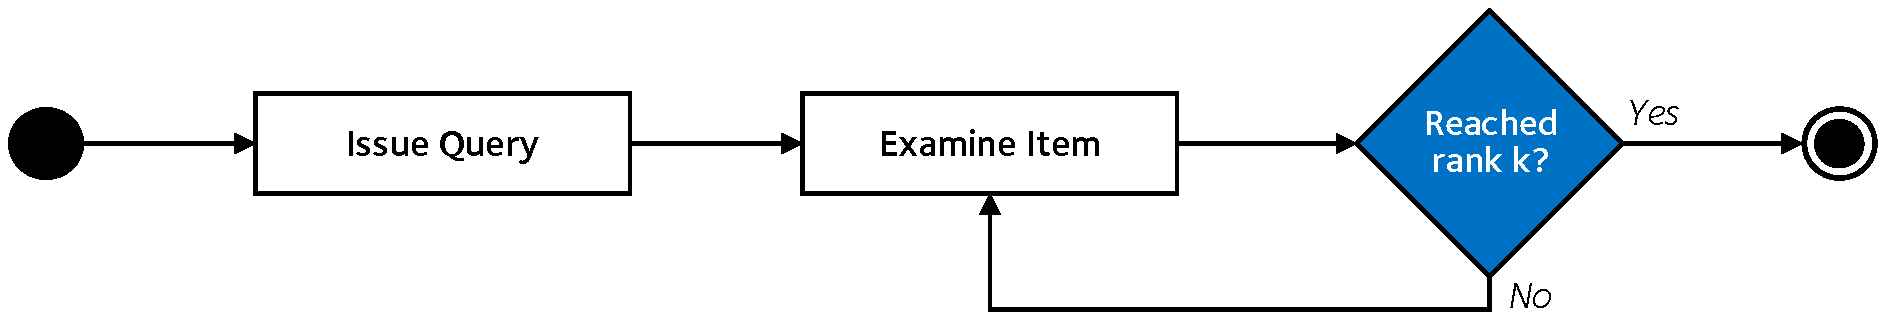
\includegraphics{figures/ch2-basic_model.pdf}}
    \caption[\gls{acr:trec} searcher model]{The~\gls{acr:trec} searcher model. Considering a highly abstracted searcher, a query is issued, with each individual result examined in a linear order, up to some depth \emph{k} (typically 1,000), before the searcher stops. No notion to relevance is considered; all documents up to rank \emph{k} are assumed by the searcher to be relevant to the topic provided.}
    \label{fig:trec_model}
\end{figure}

The basic searcher model employed by a~\gls{acr:trec}-style experiment is illustrated as a flowchart in Figure~\ref{fig:trec_model}. Given the batch-style nature of~\gls{acr:trec}-style experimentation, this particular searcher model is well suited to such an environment, as the simplifying assumptions and complete lack of interaction from the searcher go hand in hand with the design goals of the initial Cranfield II experiments, detailed in Section~\ref{sec:ir_background:paradigms} above. Searchers, when provided with an information need (or topic), will issue a single query pertaining to said information need -- the topic's title -- and then examine each individual item, one by one, considering each item as relevant to said information need. This process continues until some rank $k$, at which point the searcher will cease and the search process ends. This rank $k$ is typically set to $1,000$ to provide evaluation programs such as \texttt{trec\_eval} with a large a set of rankings as possible for accurate values for the various evaluation measures that can be computed.

With this highly abstracted searcher model being agonistic of the complex interactions that take place during search, a number of different criticisms can be made. Below, we enumerate on three primary criticisms that have been highlighted in the literature.

\begin{itemize}
    \item{\blueboxbold{A Single Query} The~\gls{acr:trec} searcher model assumes that a single query is issued for a given information need. This severely limits the potential for interaction between the searcher and retrieval system -- a single query means no \emph{query reformulation} is possible, for example. In reality, searchers \emph{do} reformulate queries, issuing multiple queries during a search session~\citep{keskustalo2009querying}.}
    \item{\blueboxbold{Assuming a Fixed Depth} Searchers subscribing to this searcher model will always examine documents to a depth of $k$. This assumes a \emph{fixed-depth stopping strategy,} where searchers are agnostic of the results as presented to them, etc. In reality, searchers adapt their stopping depths dependent upon a variety of different factors, such as the number of non-relevant items uncovered thus far~\citep{cooper1973retrieval_effectiveness_ii}.}
    \item{\blueboxbold{Everything is Inspected} The final key, limiting assumption in the~\gls{acr:trec} searcher model is that \emph{all} documents are examined and considered relevant. In reality, searchers may skim through results, or simply decide that a document does not look to be promising, and thus skip it. There is no concept of a \emph{result summary,} a shorthand overview of the contents of the document.}
\end{itemize}

Over time, researchers have begun to examine ways in which to improve upon the basic, rigid assumptions laid out by this searcher model. For example,~\cite{smucker2012tbg} introduced \emph{time-biased gain,} where probabilities of interacting with documents were included, for example. Work by~\cite{tran2017markov_models} considered the~\gls{acr:trec} searcher model from the standpoint of a Markov model, with probabilities of transitioning between different states. This work can be considered part of the study of~\gls{acr:iir}, a field that has strived to improve models of the search process, and thus improve our collective knowledge of the complex interactions that take place during search.

\subsection{Interactive Information Retrieval}\label{sec:ir_background:user:iir}
The study of~\glsfirst{acr:iir} attempt to address our lack of understanding and incorporation of a searcher's behaviours and interactions into the evaluation of retrieval systems~\citep{callan2007minds}.~\gls{acr:iir} studies can include aspects from both user-sided and system-sided research. For example, one might present results of a user study examining a particular phenomenon of a searcher's behaviour, and also provide details of a system-sided evaluation. As discussed by~\cite{kelly2009iir},~\gls{acr:iir} can trace its root back to a variety of different disciplines, including: traditional~\gls{acr:ir} (i.e. exclusively system-sided research); library and information sciences; psychology; and~\gls{acr:hci}. Typically presented as a branch of~\gls{acr:ir} and/or~\gls{acr:hci}, arguments also exist to consider~\gls{acr:iir} as a distinct area of research~\citep{ruthven2008iir}.

\begin{quote}
\emph{``In~\gls{acr:iir}, users are typically studied along with their interactions with systems and information. While classic~\gls{acr:ir} studies abstract humans out of the evaluation model,~\gls{acr:iir} focuses on users' behaviors [sic] and experiences -- including physical, cognitive and affective -- and the interactions that occur between users and systems, and users and information. In simple terms, classic~\gls{acr:ir} evaluation asks the question, does this system retrieve relevant documents?~\gls{acr:iir} evaluation asks the question, can people use this system to retrieve relevant documents?''}
\attrib{\cite{kelly2009iir}}
\end{quote}

To address the question of whether \emph{people can use a retrieval system}, we begin by examining the wider~\gls{acr:iir} process. Figure~\ref{fig:irs} on page~\pageref{fig:irs} considered a number of user-focused aspects, which are elaborated on in Figure~\ref{fig:iir}. Given some phenomenon in the natural world (perhaps by observation, reading a book, or through conversation with another human) a searcher will then begin to formulate an information need. As discussed previously in this thesis, this information need can arise from a knowledge gap in the searcher's mind, an internal inconsistency in what he or she is seeing or hearing, or a conflict of evidence. In an \emph{Anomalous State of Knowledge (ASK)}~\citep{belkin1980ask}, the searcher will then begin the~\gls{acr:iir} process, with the aim of satisfying their (perhaps vague) information need.

\begin{figure}[t!]
    \centering
    \resizebox{1\hsize}{!}{
    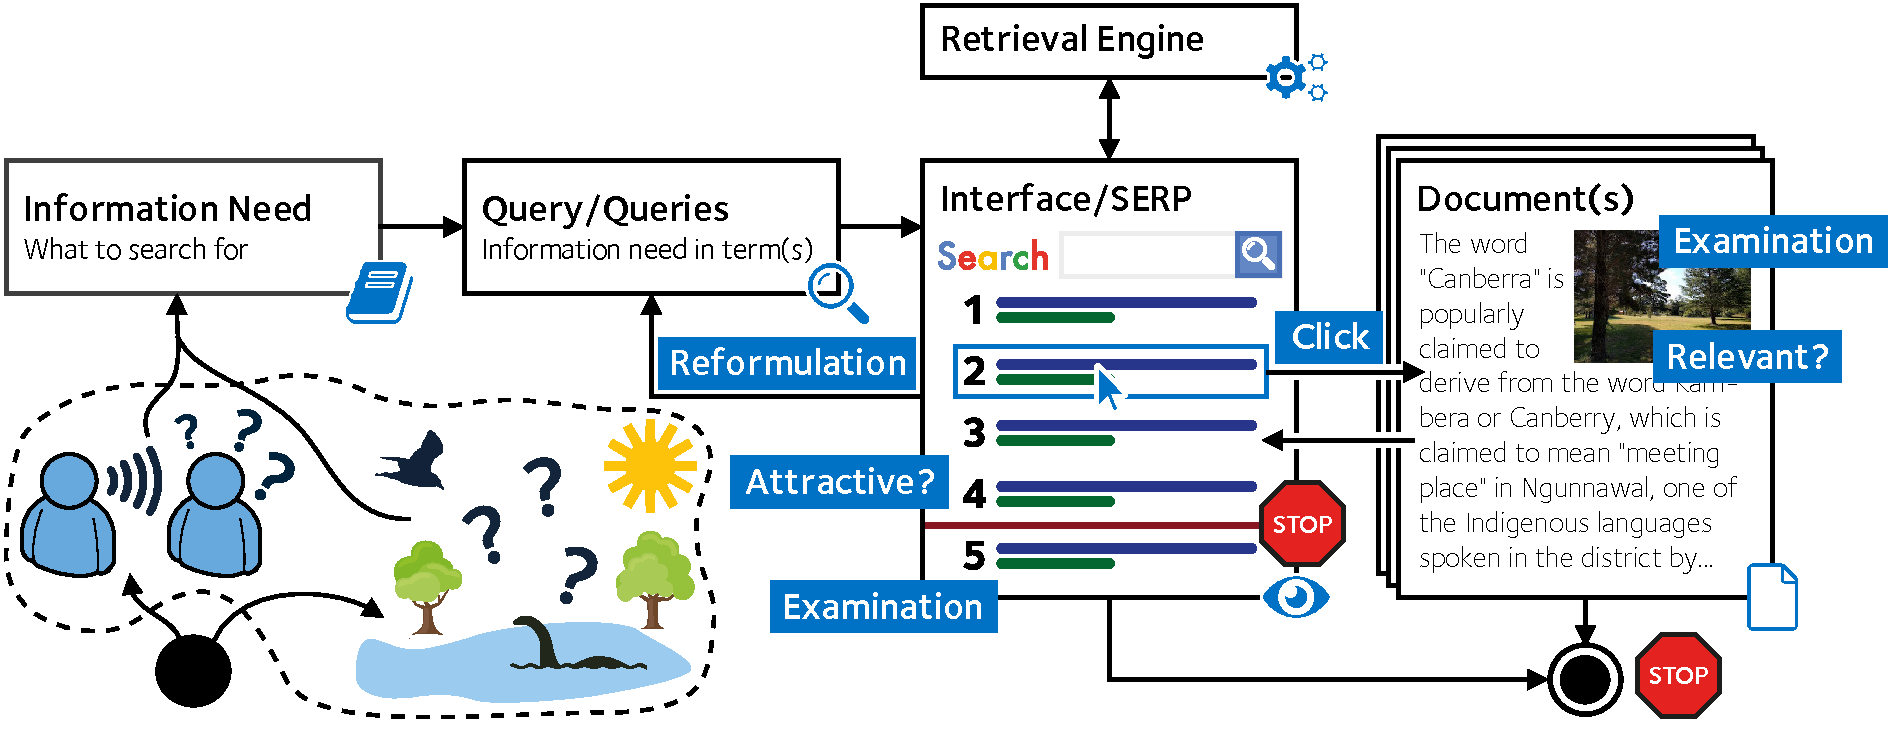
\includegraphics{figures/ch2-iir.pdf}}
    \caption[Basics of the~\gls{acr:iir} process]{Basics of the~\gls{acr:iir} process, complete with a number of different searcher interactions that can take place (although this illustration may not be exhaustive). Forming an information need, searchers then begin the interaction process by issuing a query, before examining content presented on the~\gls{acr:serp}. Searchers at given points may decide to \emph{stop} their interactions.}
    \label{fig:iir}
\end{figure}

Upon bringing up the interface of a retrieval system, the searcher begins their so-called \blueboxbold{search session}, which begins with the formulation of the information need as a series of terms -- or query. Upon submission of this query with the retrieval system, a complex series of \blueboxbold{interactions} begin to take place between the system and the searcher, and these interactions are of great importance to those studying~\gls{acr:iir}. Results will be retrieved by the underlying retrieval system and presented to the searcher in the form of a~\glsfirst{acr:serp}. While we discuss the~\gls{acr:serp} in more detail in Section~\ref{sec:ir_background:user:iir:serp}, a majority of the interactions that take place happen on the~\gls{acr:serp}.

Searchers for example will begin to examine the content on the~\gls{acr:serp}, examining individual summaries for potential relevance. At each stage, the searcher is continually learning, and thus the interaction cycle may prompt the searcher for example to provide a \emph{query reformulation} as they begin to develop their underlying mental model of the topic. A revised~\gls{acr:serp} may then begin to yield more promising results. As the searcher examines these updated results, he or she may find that a particular summary is deemed sufficiently attractive to investigate further, and thus clicks on the provided link. Taking the searcher to the corresponding document, the searcher can then examine the document in more detail, and make a decision as to its relevance. If not satisfied, the searcher may navigate back to the~\gls{acr:serp}, and continue their examination of further results. At some point, the searcher will make a decision to \blueboxbold{stop} their interactions -- either with a given~\gls{acr:serp}, or the search session as a whole (both are illustrated in Figure~\ref{fig:iir} with stop signs). Stopping may occur for example if a searcher has satisfied their information need, has been frustrated with the retrieval system's inability to return relevant results~\citep{cooper1973retrieval_effectiveness_ii}, or from a variety of different factors external to the search process, such as time pressure.

While this example above may be highly abstract in nature, it clearly shows that the search process is extremely complex and \emph{inherently interactive.} Thus, work in the field of~\gls{acr:iir} provides a basis for developing more complex, \emph{realistic} models of the search process, improving the offering when compared to the~\gls{acr:trec}-style searcher model.

\todo{WHAT ABOUT DIFFERENT TASKS?}

\subsubsection{The~\glsfirst{acr:serp}}\label{sec:ir_background:user:iir:serp}
Core to the experience of a searcher when using a given retrieval system are the interactions that take place on its~\glsplural{acr:serp}. Figure~\ref{fig:serp_example} depicts an example~\gls{acr:serp} of fictional retrieval system, \searchlogo.\footnote{We utilise \searchlogo~throughout this thesis to illustrate various concepts.} The illustration highlights several key~\gls{acr:serp} components that are extensively referred to in latter parts of this thesis. At the top of the~\gls{acr:serp} is the \blueboxbold{query box}, allowing for a searcher to reformulate their query if he or she desires.

The main body of the~\gls{acr:serp} is then divided up into the left rail and right rail. Contemporary~\glsplural{acr:serp} utilise the right rail to display additional components such as \emph{information cards} as illustrated in Figure~\ref{fig:serp_example}, and are thus become more and more complex in nature. We however in this thesis exclusively consider simplified~\glsplural{acr:serp} \emph{without} the right rail, or~\glsplural{acr:serp} comprised entirely of \emph{result summaries.}

These result summaries are typically displayed on a~\gls{acr:serp} as the \emph{ten blue links}~\citep{hearst2009_search}, or the first ten ranked results, with the document judged to be most relevant (as defined by the underlying retrieval model) displayed at the top of the list. These result summaries are short summaries of the corresponding document, and consist of three main components:

\begin{itemize}
    \item{a \blueboxbold{title} that represents the title, or headline, or a source object;}
    \item{one or more \blueboxbold{textual snippets}, providing a summary of the source object such that searchers can determine whether it is worth examining the result in more detail or not; and}
    \item{a \blueboxbold{source} for the object, typically an~\gls{acr:url} if the object is~\gls{acr:www}-based.}
\end{itemize}

\begin{figure}[t!]
    \centering
    \resizebox{1\hsize}{!}{
    
\includegraphics{figures/ch2-example.pdf}}
    \caption[Example of a~\gls{acr:serp}]{An example of a~\glsfirst{acr:serp} for the query \texttt{canberra australia}. \blueboxbold{Labels} illustrate the names of the key components of a~\gls{acr:serp} – of relevance for the work in this thesis are the \emph{result summaries.}}
    \label{fig:serp_example}
\end{figure}

Snippets are of particular interest to the work in this thesis; we explore the effect of their length on stopping behaviour in Chapter~\ref{chap:snippets}. Snippets are typically presented in contemporary retrieval systems as \emph{query-biased}~\citep{tombros1998query_biased}. This means that the snippet text relates to terms that were present in the searcher's query. Figure~\ref{fig:serp_example} demonstrates this with the use of \textbf{bolded} terms in example snippet text.

\subsection{The~\gls{acr:ir}/\gls{acr:iir} Spectrum}\label{sec:ir_background:user:spectrum}
In order to aptly describe where~\gls{acr:iir} fits into the system-sided and user-sided space,~\cite{kelly2009iir} provided an intuitive spectrum of work that bridges~\gls{acr:ir} and~\gls{acr:iir}. Figure~\ref{fig:spectrum} illustrates the spectrum, consisting of eight different categories of study. Moving from left to right in the illustration, categories shift from solely system-sided (\gls{acr:trec}-style) studies towards those that are more user focused, considering a searcher's behaviours when interacting with a retrieval system. Below, we detail three key category types as outlined by~\cite{kelly2009iir} that have particular relevance to the work detailed in this thesis.

\begin{itemize}
        \item[]{\hspace{-6mm}\raisebox{-.2\height}{
\includegraphics[height=5mm]{figures/ch2-point1.pdf}\hspace{1.5mm}}\blueboxbold{\gls{acr:trec}-Style Studies} With a majority of traditional~\gls{acr:ir} studies falling into this category,~\gls{acr:trec}-style studies focus upon the development and evaluation of system-sided research, such as retrieval models and indexing techniques. No real searchers are included \emph{in the loop} with this approach, although a simplistic, abstracted searcher model is encoded, as previously discussed in Section~\ref{sec:ir_background:paradigms:trec:model}. While assessors do create relevance judgements used for evaluation, they are not involved in the actual batch-style search process. As such, interaction is assumed to be very simplistic, with a single query issued, for example. This is illustrated in Figure~\ref{fig:trec_model} on page~\pageref{fig:trec_model}.}
    \item[]{\hspace{-6mm}\raisebox{-.2\height}{
\includegraphics[height=5mm]{figures/ch2-point2.pdf}\hspace{2mm}}\blueboxbold{'User' Relevance Assessment Studies} The second category of study does explicitly consider a human \emph{in the loop,} but only in exceptionally limited circumstances. As the name of the category suggests, the humans that are employed for this category of study are used only for generating relevance assessments, perhaps because a specific corpus is used, and no pre-existing~\gls{acr:trec} relevance assessments are available.}
    \item[]{\hspace{-6mm}\raisebox{-.2\height}{
\includegraphics[height=5mm]{figures/ch2-point5.pdf}\hspace{1mm}} \blueboxbold{\gls{acr:trec} Interactive Studies} Studies belonging to this category typically are used to evaluate a retrieval system and/or a feature of a its user interface, where and experimental retrieval system is used. Typically, aspects such as searcher behaviours, their cognition or the information seeking context are examined. These studies usually aim to assist in aiding our understanding of the search process, and the development of more intuitive and user-friendly search interfaces. Interaction is considered -- search sessions in this category of study permit searchers to issue multiple queries through query reformulation, assess documents for relevance, and conduct a number of other interactions that studies closer to the left of Figure~\ref{fig:spectrum} simply do not cater for. These studies, therefore, are more \emph{realistic} and considerate of real-world searcher behaviours.}
    
\end{itemize}

\begin{figure}[t!]
    \centering
    \resizebox{1\hsize}{!}{
    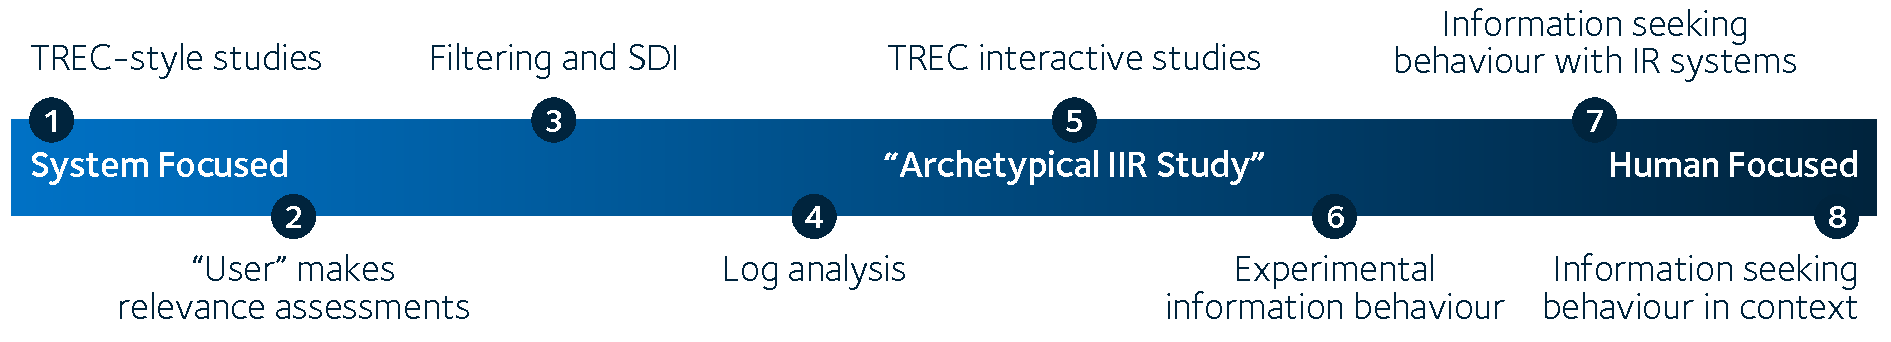
\includegraphics{figures/ch2-spectrum.pdf}}
    \caption[Spectrum IIR research~\citep{kelly2009iir}]{The spectrum of conceptualising~\gls{acr:iir} research. Methods on the left consider a more system-focused approach, with those on the right considering a more user-focused approach. The fifth step within the spectrum considering~\gls{acr:trec} interactive studies is considered to be an \emph{"archetypical~\gls{acr:iir} study"}. Figure adapted, with support from~\cite{kelly2009iir}.}
    \label{fig:spectrum}
\end{figure}

Moving to the right of the spectrum, the study of the searcher becomes ever more prominent, until we reach the following category that considers the \emph{experiences} of searchers.

\begin{itemize}
    \item[]{\hspace{-6mm}\raisebox{-.2\height}{
\includegraphics[height=5mm]{figures/ch2-point8.pdf}\hspace{1mm}} \blueboxbold{Information Seeking Behaviour in Context Studies} In this final category of study, researchers consider the information needs of individuals. Researchers would typically observe how individuals conduct their searches, while at the same time collating qualitative data about their differing experiences. These data can then be used to motivate iterations of the design and presentation of search results, thus improving the overall experience for searchers.}
\end{itemize}

The studies complying with category \raisebox{-.2\height}{
\includegraphics[height=5mm]{figures/ch2-point5.pdf}}, called \emph{archetypical~\gls{acr:iir} studies} by~\cite{kelly2009iir}, are the studies that we largely consider in this thesis. Indeed, in the contributory chapters, we consider a variety of different aspects that can influence the behaviour and performance of searchers. This work is done in combination with a series of experiments that can be considered to belong to category \raisebox{-.2\height}{
\includegraphics[height=5mm]{figures/ch2-point1.pdf}}. By \blueboxbold{grounding} these experiments with data collected from studies in category \raisebox{-.2\height}{
\includegraphics[height=5mm]{figures/ch2-point5.pdf}}, we are able to bring more realistic, credible abstractions of the search process that consider some aspects of interaction. We achieve this through \blueboxbold{simulating} the behaviour of real-world searchers to examine what happens to searcher behaviour under different contexts.

\subsection{The Simulation of Interaction}\label{sec:ir_background:user:simulation}
Simulation is defined as the \emph{imitation of the operation of a real-world process of system over time}~\citep{banks1996discrete}. Such an approach allows one to gain insight into the functioning of some real-world phenomenon, such as the complex interactions that take place during the~\gls{acr:iir} process. \emph{Computerised simulation}~\citep{heermann1990computer_simulation} has become more commonplace today with increasing computational power allowing for the development of ever more complex and realistic simulations. Indeed, simulation permits one to solve a large number of different real-world systems without resorting to a \emph{``bag of tricks''}~\citep{fishwick1995simulation}, where special purpose (and often arcane) solutions must be used. Such an example could be s a series of linear equations~\citep{fishwick1995simulation}. With this a \emph{closed-form} approach, underlying assumptions can become twisted and altered to suit such an approach, drifting the representation further away from the real-world phenomenon being considered.

Simulation avoids such issues by providing one with the freedom and flexibility to reduce these assumptions that may otherwise be included. This permits a rapid means of exploring different scenarios, all at a low cost. Additionally, without needing to consider issues such as subject fatigue (within a user study, for example), simulation provides the capability of running experiments with reproducible results~\citep{azzopardi2010workshop}. 

Simulation has been employed extensively within classical~\gls{acr:ir} experimentation.\footnote{For an in-depth discussion of various classical~\gls{acr:ir} simulations, refer to~\cite{heine1981simulation}.}~\gls{acr:trec}-style experimentation can be considered as a form of simulation, where the simple searcher model discussed in Section~\ref{sec:ir_background:paradigms:trec:model} is used to simulate the searcher's interactions. We consider in this thesis the \emph{simulation of interaction,} where one attempts to mimic behaviours that a searcher exerts when interacting with a retrieval system~\citep{azzopardi2010workshop}. This means that we can explore different searcher behaviours, methods and techniques to better understand how searchers do, could, or are likely to behave. However, such simulations are questionable and open to criticism if they are not properly motivated, grounded and validated. There is therefore a pertinent need to ensure that such simulations are credible abstractions of the search process, and that they are seeded with data based on actual human interaction data (study category \raisebox{-.2\height}{
\includegraphics[height=5mm]{figures/ch2-point5.pdf}}, as per Section~\ref{sec:ir_background:user:spectrum})~\citep{azzopardi2010workshop}.\footnote{An exception to this rule would be the exploration of \emph{what-if} scenarios, allowing researchers to examine \emph{what} would happen to a searcher's behaviour \emph{if} a particular scenario were to be applied. One example of such a study is that by~\cite{azzopardi2011economics}.} Such grounding can for example permit \emph{stochastic simulations,} working on the notion of the \emph{probabilities of interaction} (e.g. the probability of clicking on a relevant result summary).

Within the wider~\gls{acr:iir} process, a number of different individual components have been examined through use of simulation. These have often been independently analysed from one another~\citep{azzopardi2010workshop}, with examples of different components and associated studies listed below.

\begin{itemize}
    \item{\blueboxbold{Query Formulation and Suggestions} This component considers querying, including the generation of pseudo-realistic queries and the development of realistic \emph{querying strategies,} grounded upon the querying behaviours of real-world subjects. Examples include studies by:~\cite{azzopardi2009query_side, azzopardi2007languages, carterette2015test_collections, jordan2006cqg, keskustalo2009querying} and~\cite{verberne2015personalised_queries}.}
    
    \item{\blueboxbold{Browsing Behaviours} This broader component considers the wider behaviours of searchers when examining content, including aspects such as click models, and different browsing strategies employed by searchers (e.g. can a searcher's behaviour as \emph{fast and liberal,} or \emph{slow and neutral} -- as outlined by~\cite{smucker2011user_strategies}). In addition to the work by~\cite{smucker2011user_strategies}, examples include~\cite{carterette2015test_collections, chuklin2015click_models, guo2009click_chain}; and~\cite{pakkonen2015behavioural_dimensions}.}
    
    \item{\blueboxbold{The Influences of Cost and Time} This component examines how varying \emph{interaction costs} (i.e. the cost of issuing a query, or examining a document, considered primarily in terms of the amount of time required) and time constraints can influence the behaviour of searchers. Examples include the economics-based approach outlined by~\cite{azzopardi2011economics}, and work by~\cite{baskaya2012simulating_sessions}.}
    
    \item{\blueboxbold{Performance over Search Sessions} This area of work considers how, when different aspects are changed, the performance of a searcher over a search session varies. Examples include work by~\cite{luo2014winwin} and~\cite{luo2015pomdp}.}
\end{itemize}

Of particular relevance to this thesis is the work that has been undertaken to examine a searcher's \blueboxbold{stopping behaviour}, with examples including:~\cite{carterette2011models, carterette2015test_collections, maxwell2015initial_stopping, maxwell2015stopping_strategies}; and~\cite{thomas2014modelling_behaviour}. In these works, different \emph{stopping strategies} and \emph{stopping models} are proposed. These are considered in depth later in Chapter~\ref{chap:stopping_background}.

Simulation provides a means for examining the aforementioned components from two different standpoints:

\begin{itemize}
    \item{considering each of the individual components in isolation (e.g. exclusively examining querying behaviours); or}
    \item{considering the interactive search process as a whole, and attempting to capture and model an entire search session, from querying to document examination.}
\end{itemize}

The work in this thesis considers the latter, or the entire search process, meaning that potential influences of components over others can be considered. This also justifies the need for a more advanced searcher \emph{model} that captures the interactions of the wider search process. A model is a key component of a simulation, or the representation of the real-world phenomenon being simulated~\citep{tocher1963art_of_simulation}. With the~\gls{acr:trec}-style searcher model outlined, we turn our attention to considering more advanced searcher models of the~\gls{acr:iir} process.

\subsection{Searcher Models}\label{sec:ir_background:user:models}
Models of the search process attempt to capture the high level, cognitive processes that a searcher undertakes during a search session -- such as issuing a query, or examining a document for relevance. As we have discussed previously, highly abstracted searcher models have been present in system-sided~\gls{acr:ir} research, as well as implicitly encoded within a variety of different evaluation measures, as discussed in Section~\ref{sec:ir_background:evaluation}.

\cite{carterette2011effectiveness_evaluation} argues that the measures widely used within~\gls{acr:ir} research are themselves typically comprised of three distinct underlying models that are enumerated below.

\begin{itemize}
    \item{\blueboxbold{Browsing Model} Browsing models describe how a searcher interacts with a retrieval system's interface, including the~\glsplural{acr:serp} that are presented to them.}
    \item{\blueboxbold{Document Utility Model} These models encode some form of \blueboxbold{document utility} that provides a description for how utility or \emph{gain} can be derived from relevant documents; and}
    \item{\blueboxbold{Utility Accumulation Model} This final model describes how a searcher accumulates said utility over the course of an entire search session.}
\end{itemize}

Of particular interest to the work in this thesis are the browsing models that attempt to capture the broad array of interactions that take place between the searcher and the search engine. The~\gls{acr:trec} searcher model is a high abstracted example of such a model, yet there is a disconnect between the assumptions made in this searcher model and reality. As such, we now discuss a number of more advanced searcher models, providing better representations of the complex interactions that take place during~\gls{acr:iir}.

Seminal work undertaken by~\cite{baskaya2013behavioural_factors} presented an explicit, revised searcher model that improved upon the \emph{interactive} capabilities that could be exploited. Improvements over the~\gls{acr:trec}-style searcher model included the following:

\begin{itemize}
    \item{the ability to \blueboxbold{separately judge result summaries} presented on a~\gls{acr:serp} from the documents associated with each;}
    \item{permitting a searcher the ability to \blueboxbold{stop at a variable depth on the~\gls{acr:serp}}, avoiding fixed depth stopping behaviours as typically employed in searcher models; and}
    \item{permitting a searcher to \blueboxbold{issue multiple queries} during a search session, lifting one of the major constraints of the~\gls{acr:trec} searcher model.}
\end{itemize}

These improvements are demonstrated as a Markov model, illustrated in Figure~\ref{fig:baskaya_model}. Compared to the~\gls{acr:trec}-style searcher model illustrated in Figure~\ref{fig:trec_model} on page~\pageref{fig:trec_model}, the model can be visually seen as more complex, consisting of six main actions:

\begin{itemize}
    \item{\blueboxbold{query formulation}, where a searcher formulates the terms that they wish to enter, as well as the issuance of the query to the underlying retrieval system;}
    \item{\blueboxbold{snippet scanning}, the action that considers the examination of individual result summaries for \emph{attractiveness;}}
    \item{\blueboxbold{link clicking} that occurs when a result summary is considered to be attractive enough to warrant further examination;}
    \item{\blueboxbold{document examination} that considers the process of examining a document for relevance to the underlying information need;}
    \item{\blueboxbold{relevance judging}, for determining whether or not the document is relevant to the searcher's information need; and}
    \item{\blueboxbold{session stopping}, the action that curtails the search session.}
\end{itemize}

These steps broadly match up the~\gls{acr:iir} process as outlined in Figure~\ref{fig:iir} on page~\pageref{fig:iir}, and described in abstract form in Section~\ref{sec:ir_background:user:iir}.~\cite{azzopardi2011economics},~\cite{yilmaz2010browsing_utility},~\cite{carterette2011models}, and more recently~\cite{zhang2017simulation_model} have all introduced and utilised searcher models that are similar in terms of the broad set of actions as outlined by~\cite{baskaya2013behavioural_factors}. Being a Markov model, this searcher model considers each of the different actions as a \emph{state} within the model, with a series of \emph{transition probabilities} linking each of the actions together (i.e. \emph{what is the probability of a searcher moving from scanning a snippet to stopping the search session?)}.\footnote{This searcher model can also be represented as a flowchart, as illustrated in Figure~\ref{fig:baskaya_model_flow}.} Indeed, the typical browsing model components (e.g. inspecting a document for relevance) as per~\cite{carterette2011effectiveness_evaluation} are also integrated with query generation and utility accumulation, allowing a searcher to issue multiple queries and gain utility.

\begin{figure}[t!]
    \centering
    \resizebox{1\hsize}{!}{
    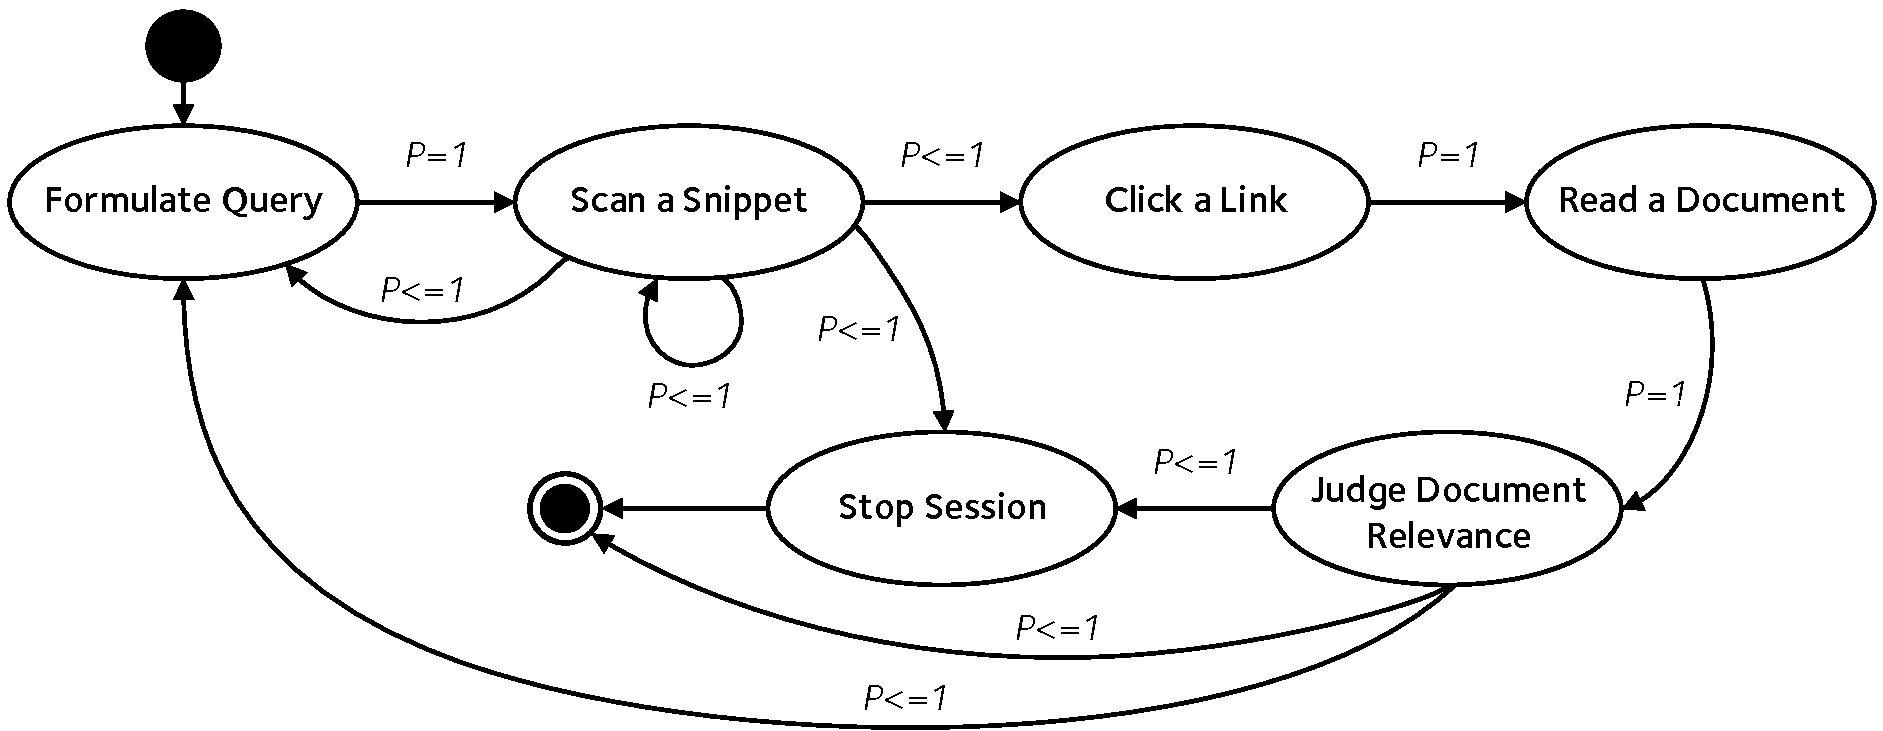
\includegraphics{figures/ch3-baskaya.pdf}}
    \caption[Markov model of the search process by~\cite{baskaya2013behavioural_factors}]{The user model of search, as outlined by~\citealt{baskaya2013behavioural_factors}. Represented as a Markov model, the model considers six steps in all. Encoded within two of the steps are decision points that a user following this model must consider in order to continue. Figure adapted with the support from the authors of~\citealt{baskaya2013behavioural_factors}.}
    \label{fig:baskaya_model}
\end{figure}

\begin{figure}[t!]
    \centering
    \resizebox{1\hsize}{!}{
    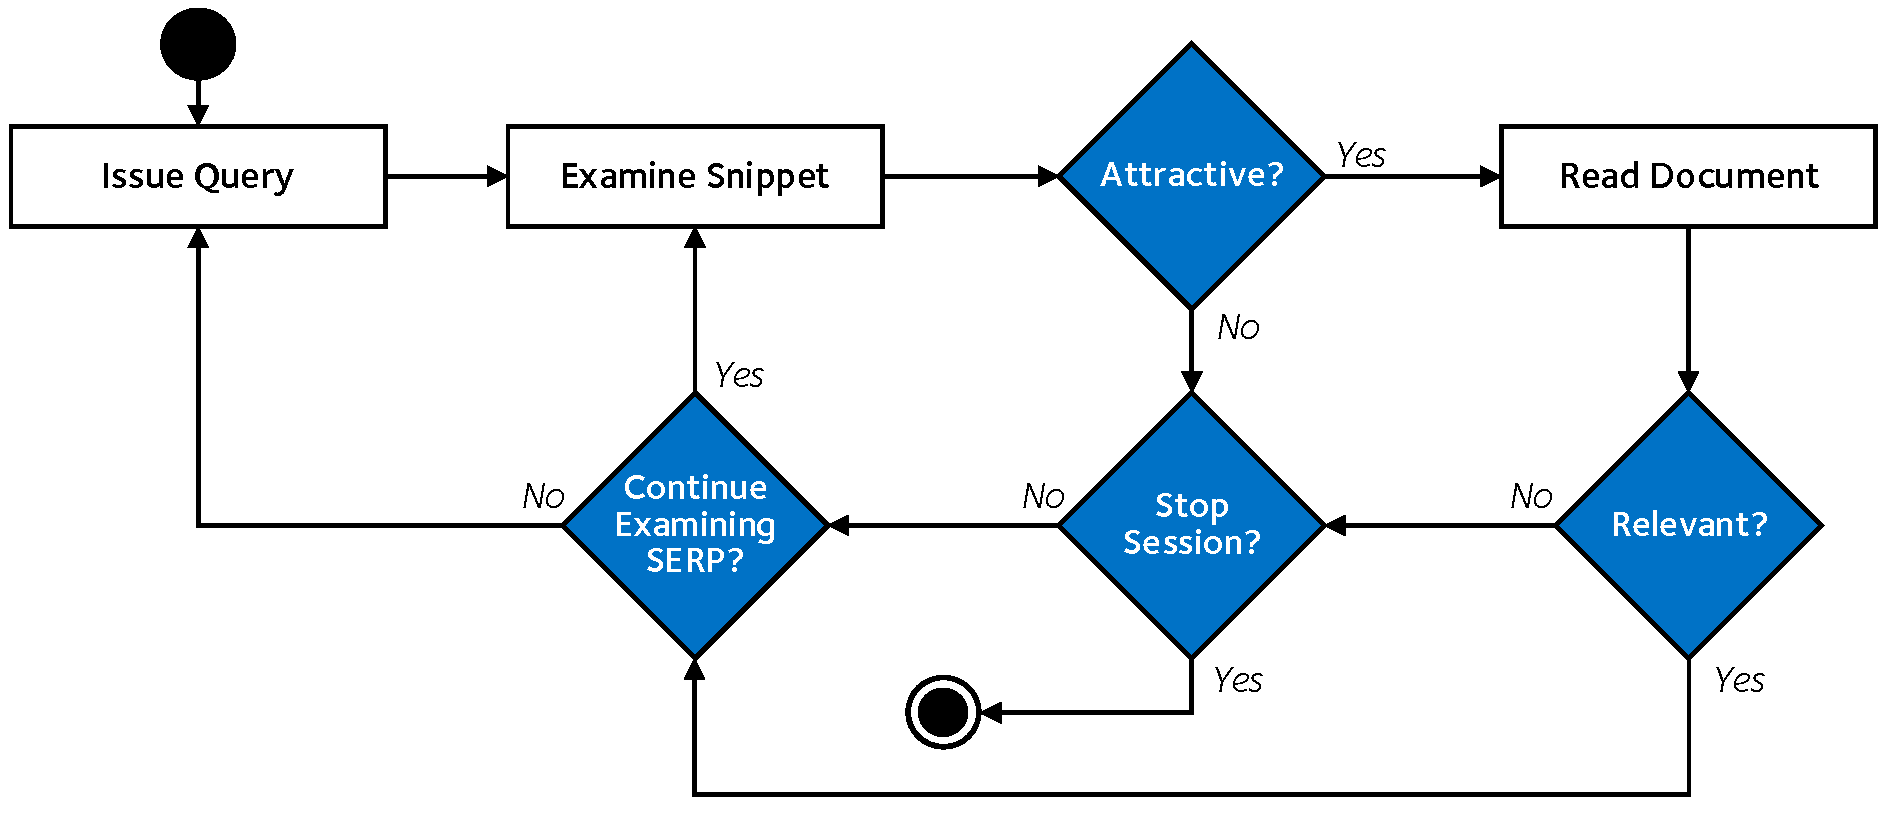
\includegraphics{figures/ch3-baskaya_flow.pdf}}
    \caption[Flowchart of the search process by~\cite{baskaya2013behavioural_factors}]{The user search model, as outlined by~\cite{baskaya2013behavioural_factors}. Adapted from the version of the model illustrated later in Figure~\ref{fig:baskaya_model}, this flowchart illustrates the main processes, decisions and interaction flow that an individual subscribing to this model will follow.}
    \label{fig:baskaya_model_flow}
\end{figure}

Judging result summaries separately from the associated documents is to be regarded as a major development in searcher models. The snippet text forming part of each result summary can be generated in a variety of different ways, with approaches today typically \emph{query biased} in nature~\citep{tombros1998query_biased}. As such, what may look like a result summary that is attractive enough to explore further could potentially lead to a document that is in actuality not pertinent to the given information need. This is a clear development from the~\gls{acr:trec}-style searcher model that doesn't even consider the notion of a result summary.

Effectively modelling stopping behaviour is also important to providing a more realistic model of the search process. The addition of decision points allowing a searcher to judge the attractiveness of a snippet, or the relevancy of a document, provide natural locations for stopping decision points.

\begin{quote}
\emph{Given this snippet looks unattractive and therefore not useful to satisfying my information need, should I stop examining the results presented to me on this~\gls{acr:serp}?}
\end{quote}

\begin{figure}[t!]
    \centering
    \resizebox{1\hsize}{!}{
    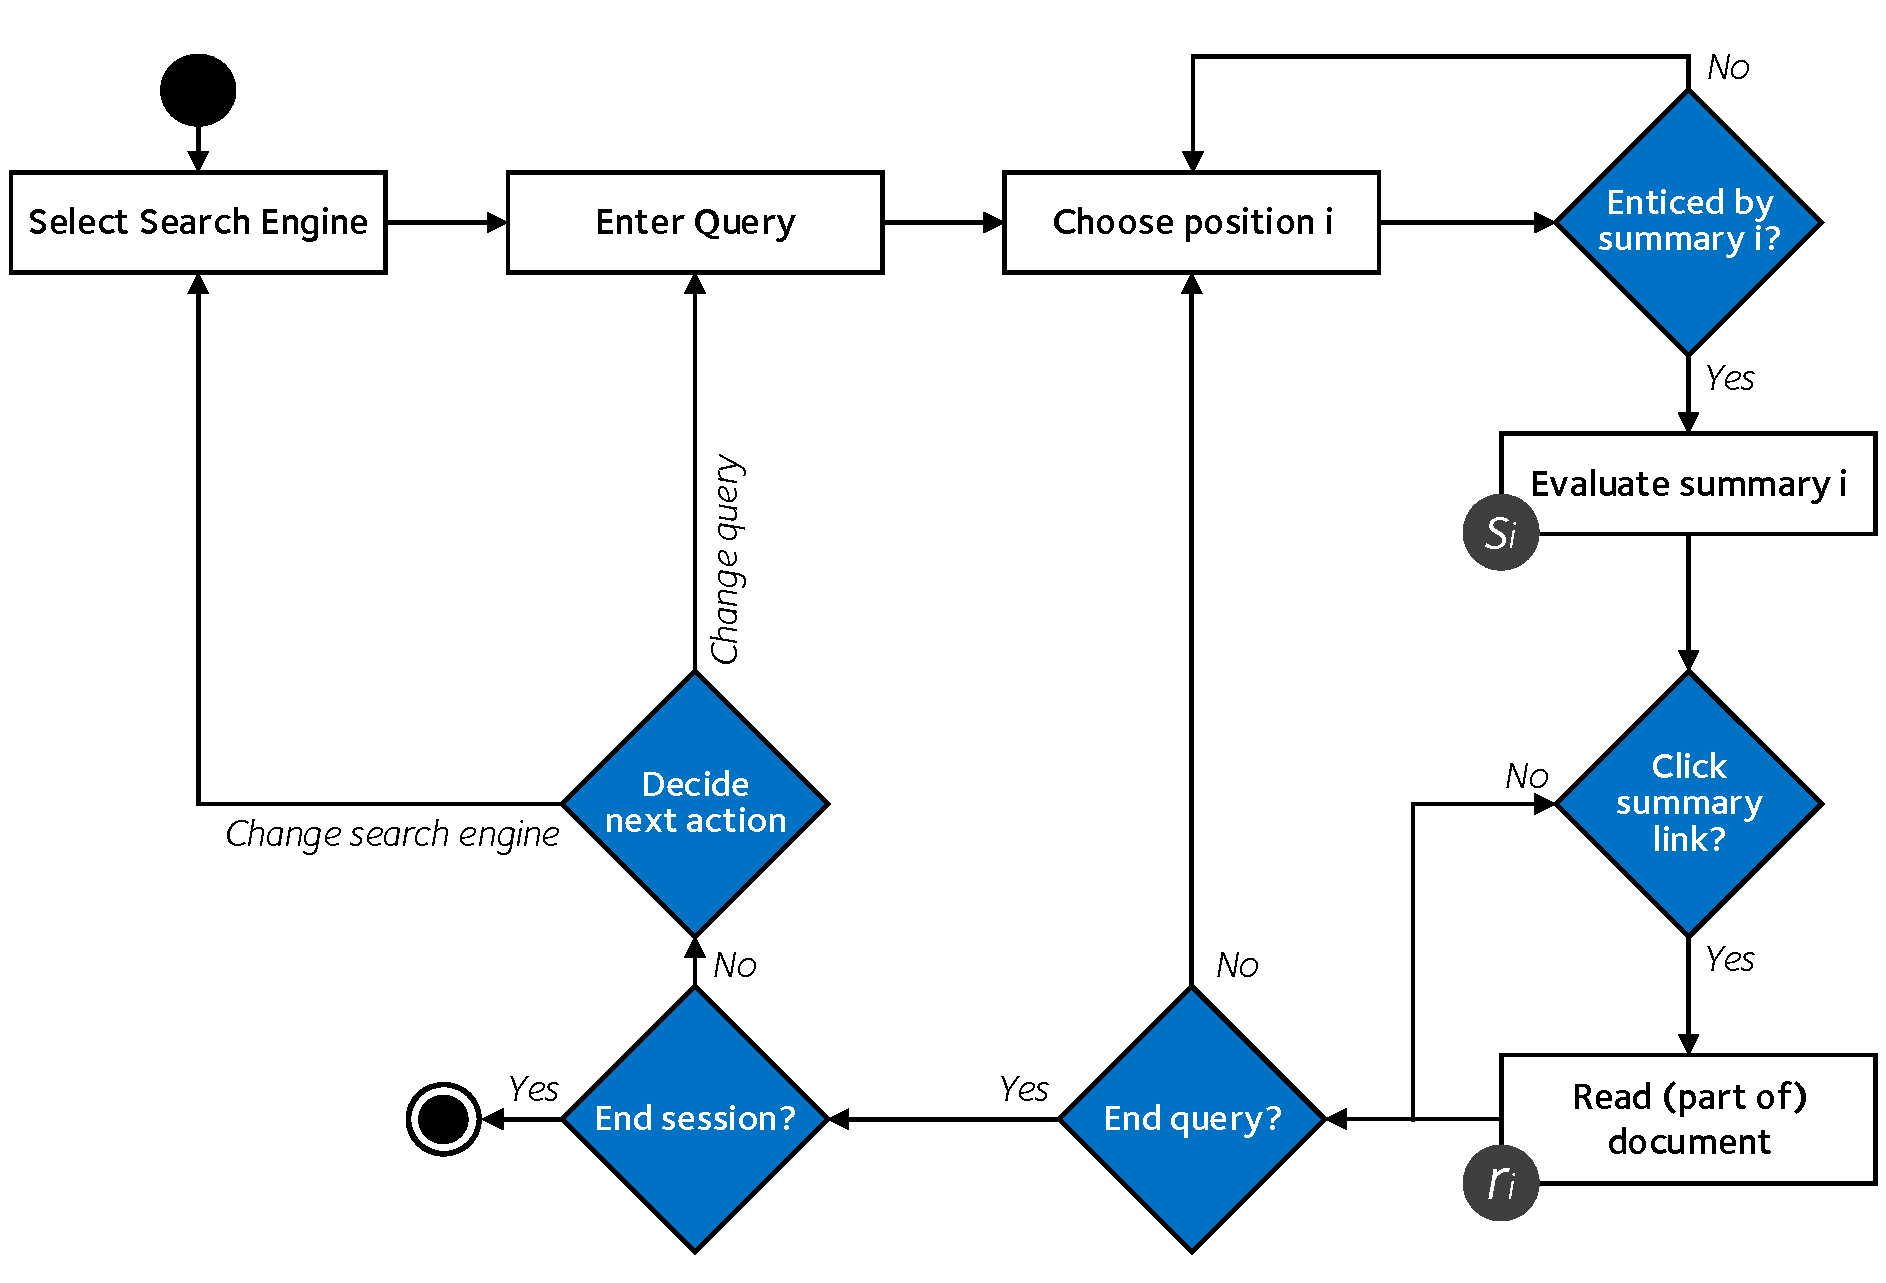
\includegraphics{figures/ch3-thomas.pdf}}
    \caption[Model of the search process by~\cite{thomas2014modelling_behaviour}]{A model of the search process, considering the high-level processes undertaken by a searcher, as outlined by~\cite{thomas2014modelling_behaviour}. Figure adapted, with the support of the authors Thomas, Moffat, Bailey and Scholer.}
    \label{fig:thomas_model}
\end{figure}

As an example, a searcher may issue a query that returns very few relevant documents. Once a few snippets and/or documents have been examined, he or she will then conclude that the issued query was unsuccessful, and that they would be essentially wasting their time examining more content on the present~\gls{acr:serp}. In this case, issuing a reformulated query would be a better course of action. This intuition has been confirmed by empirical analysis, where~\cite{azzopardi2011economics} demonstrated that simulated searchers examined significantly fewer documents when the underlying search engine failed to retrieve any relevant material in the top ten results, in contrast to when they did. Thus, searchers are inherently adaptive, with their behaviours conditioned upon the quality of the ranked lists that they interact with. This justifies the inclusion of these additional stopping decision points.

A further explicitly defined searcher model was proposed by~\cite{thomas2014modelling_behaviour}. This model, illustrated as a flowchart in Figure~\ref{fig:thomas_model}, encapsulates the same principles as the previously described searcher models: given an information need, a searcher will issue one or more queries, and examine a varying number of result summaries and documents for attractiveness and relevance respectively. This searcher model also includes a form of utility accumulation model that considers the utility obtained from a result summary $s_i$ and the relevancy judgement of a document, $r_i$. An addition to this searcher model is the inclusion of an additional step at the beginning of the search session, where a searcher must decide \emph{what retrieval system to use.} This may be dependent upon the task at hand: a patent retrieval system would be a better bet for finding associated patents as opposed to a general web retrieval system, for example.

The searcher model proposed by~\cite{thomas2014modelling_behaviour} also considers the examination of result summaries from a different perspective. Instead of assuming that a searcher (perhaps na\"{i}vely) examines each individual result summary in detail before making a decision to its attractiveness, searchers subscribing to this searcher model undertake an \emph{initial inspection} of result summaries, where they can examine in either direction on the list of ranked results (by increasing or decreasing some positional counter, $i$). Essentially, this can be regarded as a searcher \emph{skimming} result summaries, determining if they are worthy of further examination.

Despite the slight variations in how different researchers interpret the~\gls{acr:iir} process, what can be clearly seen from examination of the models discussed in this section is a similar workflow between each. From query issuance to document examination and judgement, this has emerged as the generally accepted process of~\gls{acr:iir}. While studies examining explicit searcher models are not common, searcher models have been encoded within many of the different evaluation measures used within~\gls{acr:ir} and~\gls{acr:iir}. Moving onto the final section of this background chapter, this is now what we turn our attention towards.

\section{Evaluation Measures}\label{sec:ir_background:evaluation}

\subsection{System-Based Evaluation}\label{sec:ir_background:evaluation:system}

\subsubsection{Precision}

\subsubsection{Recall}

\subsubsection{Mean Average Precision}

\subsubsection{Expected Search Length}

\subsection{Searcher-Based Evaluation}

\subsubsection{Interactive Precision and Recall}

\subsubsection{Cumulative Gain Measures}

\subsubsection{Rank-Biased Precision}

\subsubsection{INST}

\section{Chapter Summary}